\RequirePackage[l2tabu,orthodox]{nag}

\documentclass[headsepline,footsepline,footinclude=false,oneside,fontsize=11pt,paper=a4,listof=totoc,bibliography=totoc]{scrbook} % one-sided

\PassOptionsToPackage{table,svgnames,dvipsnames}{xcolor}

\usepackage[utf8]{inputenc}
\usepackage[T1]{fontenc}
\usepackage[sc]{mathpazo}
\usepackage[ngerman,american]{babel}
\usepackage[autostyle]{csquotes}
\usepackage[%
  backend=biber,
  url=false,
  style=alphabetic,
  maxnames=4,
  minnames=3,
  maxbibnames=99,
  giveninits,
  uniquename=init]{biblatex}
\usepackage{graphicx}
\usepackage{scrhack} % necessary for listings package
\usepackage{listings}
\usepackage{lstautogobble}
\usepackage{tikz}
\usepackage{pgfplots}
\usepackage{pgfplotstable}
\usepackage{booktabs}
\usepackage[final]{microtype}
\usepackage{caption}
\usepackage{amsmath}
\usepackage{algorithmic}
\usepackage{algorithm}
\usepackage[hidelinks]{hyperref} % hidelinks removes colored boxes around references and links

\bibliography{bibliography}

\setkomafont{disposition}{\normalfont\bfseries} % use serif font for headings
\linespread{1.05} % adjust line spread for mathpazo font

% Add table of contents to PDF bookmarks
\BeforeTOCHead[toc]{{\cleardoublepage\pdfbookmark[0]{\contentsname}{toc}}}

% Define TUM corporate design colors
% Taken from http://portal.mytum.de/corporatedesign/index_print/vorlagen/index_farben
\definecolor{TUMBlue}{HTML}{0065BD}
\definecolor{TUMSecondaryBlue}{HTML}{005293}
\definecolor{TUMSecondaryBlue2}{HTML}{003359}
\definecolor{TUMBlack}{HTML}{000000}
\definecolor{TUMWhite}{HTML}{FFFFFF}
\definecolor{TUMDarkGray}{HTML}{333333}
\definecolor{TUMGray}{HTML}{808080}
\definecolor{TUMLightGray}{HTML}{CCCCC6}
\definecolor{TUMAccentGray}{HTML}{DAD7CB}
\definecolor{TUMAccentOrange}{HTML}{E37222}
\definecolor{TUMAccentGreen}{HTML}{A2AD00}
\definecolor{TUMAccentLightBlue}{HTML}{98C6EA}
\definecolor{TUMAccentBlue}{HTML}{64A0C8}

% Settings for pgfplots
\pgfplotsset{compat=newest}
\pgfplotsset{
  % For available color names, see http://www.latextemplates.com/svgnames-colors
  cycle list={TUMBlue\\TUMAccentOrange\\TUMAccentGreen\\TUMSecondaryBlue2\\TUMDarkGray\\},
}

% Settings for lstlistings
\lstset{%
  basicstyle=\ttfamily,
  columns=fullflexible,
  autogobble,
  keywordstyle=\bfseries\color{TUMBlue},
  stringstyle=\color{TUMAccentGreen}
}


% TODO: spelling mistake
\newcommand*{\getUniversity}{Technische Universität München}
\newcommand*{\getFaculty}{Department of Informatics}
\newcommand*{\getTitle}{Development of a Recommender System that addresses the diversity principle to improve user satisfaction.}
\newcommand*{\getTitleGer}{Entwicklung eines Empfehlungdienst unter Berücksichtigung der Benutzerzufriedenheit zur Diversität der Empfehlungen.}
\newcommand*{\getAuthor}{Ozan Pekmezci}
\newcommand*{\getDoctype}{Master's Thesis in Informatics}
\newcommand*{\getSupervisor}{Prof. Dr-Ing. Klaus Diepold}
\newcommand*{\getAdvisor}{Julian Wörmann, M.Sc.}
\newcommand*{\getSubmissionDate}{15.05.2019}
\newcommand*{\getSubmissionLocation}{Munich}

\begin{document}

% Set page numbering to avoid "destination with the same identifier has been already used" warning for cover page.
% (see https://en.wikibooks.org/wiki/LaTeX/Hyperlinks#Problems_with_Links_and_Pages).
\pagenumbering{alph}
\begin{titlepage}
  % HACK for two-sided documents: ignore binding correction for cover page.
  % Adapted from Markus Kohm's KOMA-Script titlepage=firstiscover handling.
  % See http://mirrors.ctan.org/macros/latex/contrib/koma-script/scrkernel-title.dtx,
  % \maketitle macro.
  \oddsidemargin=\evensidemargin\relax
  \textwidth=\dimexpr\paperwidth-2\evensidemargin-2in\relax
  \hsize=\textwidth\relax

  \centering

  \IfFileExists{logos/tum.pdf}{%
    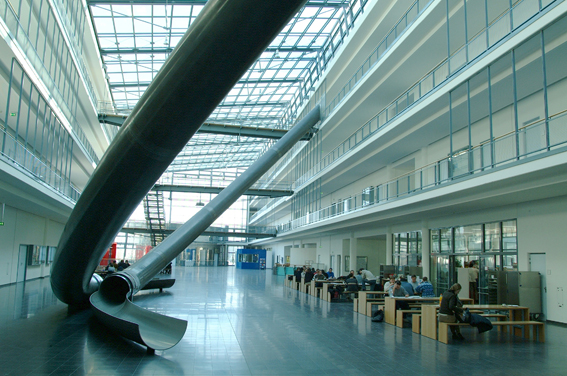
\includegraphics[height=20mm]{logos/tum.pdf}
  }{%
    \vspace*{20mm}
  }

  \vspace{5mm}
  {\huge\MakeUppercase{\getFaculty{}}}\\

  \vspace{5mm}
  {\large\MakeUppercase{\getUniversity{}}}\\

  \vspace{20mm}
  {\Large \getDoctype{}}

  \vspace{15mm}
  {\huge\bfseries \getTitle{}}

  \vspace{15mm}
  {\LARGE \getAuthor{}}

  \IfFileExists{logos/faculty.png}{%
    \vfill{}
    
\includegraphics[height=20mm]{logos/faculty.png}
  }{}
\end{titlepage}


\frontmatter{}

\input{pages/title}
\input{pages/disclaimer}
\addcontentsline{toc}{chapter}{Acknowledgments}
\thispagestyle{empty}

\vspace*{20mm}

\begin{center}
{\usekomafont{section} Acknowledgments}
\end{center}

\vspace{10mm}

Throughout the writing of this thesis, I have received a great deal of support and assistance. I would first like to thank the company Motius for supporting me in the evaluation and providing me the dataset.

I want to acknowledge my supervisor, Professor Diepold, for accepting my thesis topic.

I would also like to thank Julian Wörmann, who guided me, brainstormed with me, showed interest, and gave feedback about my thesis. I wish him the best with his career as a doctor and also on his new adventure with his family.

Besides, I would like to thank my parents, Zübeyde and Necmi Pekmezci. I would not be here without your emotional and financial support from the day that I was born.

I want to thank my girlfriend, Cosku Özdemirci, who reminded me how to feel emotions and made life more bearable.

I also want to thank my Munich friends for making life more enjoyable, especially Berkay Soykan, Haydar Sahin, Helin Senbayram, Ulas Özdemirci, Zeynep Sasi and Zeynep Karagoz, who gave me the idea of using this section more productively.

My long-distance friends Ada Gencoglu and Ugur Kocak also supported me emotionally, and I am thankful for having them in my life.

I want to offer special thanks to Akin Akkan, who, although no longer with us, our memories will be in my mind until I die.

I also want to thank some people that I do not know personally: thanks to the organizers of the Fusion Festival for teaching how to resist against the authority when needed and I want to thank the elected mayor of Istanbul, Ekrem Imamoglu, for giving me motivation, hope and showing me how to combat without being exclusive or hostile.

Everything is going to be great!


\cleardoublepage{}

\chapter{\abstractname}

Recommendation systems have an essential aim of increasing user satisfaction. However, many developers of these systems do not take into account that user satisfaction does not only depend on simple evaluation metrics like accuracy, but it can also depend on privacy, data security, diversity, serendipity, labeling, and presentation.

This work aimed to find answers to three main questions. The first question is whether high accuracy guarantees high user satisfaction. The second is an extension of the first question and asks if diversity has a positive impact on user satisfaction. The last question asks if a feedback loop increases user satisfaction.

To answer these questions, we have developed models and algorithms to generate predictions. Then we implemented these models and algorithms in a dashboard. Most recently, we conducted offline and online evaluation rounds and user studies to validate our hypothesized questions. First, we have seen that high accuracy does not always result in high user satisfaction. This is because other properties can also affect user satisfaction and a slight increase in accuracy can lead to a reduction in other properties that can also reduce user satisfaction. These properties can vary from setting to setting and from application to application. We have found that diversity is a critical factor in our use-case, which is the recommendation of a group of talents for a project. Although accuracy and diversity are inversely proportional, a slight increase in diversity led to slightly higher user satisfaction. However, a significant increase in diversity led to a decline in user satisfaction. Last, we checked if a feedback loop increases user satisfaction. Although initial implementation and training with a feedback loop does not increase user satisfaction, subjects in the user study reported more positive feedback after more and more feedback. After inserting more than a thousand feedbacks and re-training with the resulting data, users were happier with the results. We have concluded that user satisfaction in recommender systems can be increased if developers take user feedback into account and not solely focus on algorithmic accuracy.

It is hoped this thesis will inform researchers and developers of recommender systems about increasing user satisfaction.

Keywords: recommendation systems, accuracy, diversity, evaluation properties, group recommendations, job recommender system



\microtypesetup{protrusion=false}
\tableofcontents{}
\microtypesetup{protrusion=true}

\mainmatter{}

% !TeX root = ../main.tex
% Add the above to each chapter to make compiling the PDF easier in some editors.
% Add the below not to get bullet point font warnin
\renewcommand\textbullet{\ensuremath{\bullet}}

\chapter{Introduction}\label{chapter:introduction}

The introduction chapter of the thesis will focus on explaining the basic terminology of recommender systems so that readers who are new to the topic can understand the rest quickly. In addition to that, we will also present the motivation and the hypotheses that we want to validate.

\section{Recommender Systems}

"Recommender Systems are software tools and techniques that provide suggestions for items that are most likely of interest to a particular user." ~\parencite{Ricci2015}

Suggestions and items depend on the field that the recommender system is applied. For example, for the topic of news article recommenders, the aim will most likely be suggesting news to the readers. In the field of job recommenders though, these suggestions can be bidirectional. Meaning that job postings can be suggested to applicants or resumes can be recommended to the human resources team of a company.

Although the history of the recommender systems goes back to mid-1990s ~\parencite{PARK201210059}, the real boom happened after e-commerce services became mainstream \cite{smith2017two}. Since there were too many items to choose from for users, such service was needed. Users of websites were becoming overloaded with the information, and the developers of recommender systems had the aim of reducing the information to be only relevant to users. 

\section{Why Recommender Systems?}

As mentioned in the last paragraph, recommender systems have the general function of suggesting items to users. However, why do recommender systems get developed? What kind of benefit do they have for both companies and users?

First of all, recommender systems increase the number of items sold  ~\parencite{Ricci2015}.  Also, most recommenders suggest personalized results, which means that users will see content that fits their desires. These recommendations will also increase users buying more items.

Recommenders also increase the coverage of items that user see. Coverage denotes the number of recommended unique items divided by the number of all items. Therefore, users can interact with items that they would not even see without recommenders, that improves the chances of buying more items.

Another essential point is increasing user satisfaction. This function of recommenders is the foundation of the thesis at hand. Unfortunately, most of the researchers do not take into account that the user satisfaction does not solely depend on simple evaluation metrics like accuracy, precision or recall but it can also depend on privacy, data security, diversity, serendipity, labeling, and presentation ~\parencite{Beel2016}. When recommender systems take those factors into account, they increase user satisfaction.

\section{User Satisfaction}

The recommendation performance is mainly evaluated in terms of accuracy (i.e., the difference between actual and predicted rating). Concentrating on the accuracy might not be a desired goal of the talent/project recommendations (e.g., merely recommending a \textit{top-N} list of talents that best match the requirements might result in similar talents whose skills only vary in a small extent). Besides the desired diversity, there might be other properties necessary for adequate recommendations (e.g., privacy, data security, diversity, serendipity, labeling, and presentation, and group recommendation).

\section{Setting}

Recommender systems can be applied to a various set of fields like entertainment, content creation, e-commerce, service sector, and social. However, we chose specific use-case, which is the suggestion of talents to projects to be managed by the recruiters of the companies.

\section{Datasets}\label{section:intro-datasets}

To be able to develop a solution on this topic, we used two datasets: one from the website \textit{Freelancer.com} and another one from the company \textit{Motius Gmbh}. These datasets are presented in the section \ref{section:datasets}.


\section{Motivation}\label{section:motivation}

This thesis aims to find answers to three main questions. The first question is if high accuracy guarantees high user satisfaction. The second one is an extension to the first question and asks if diversity affects user satisfaction positively. The last question asks if a feedback loop increases user satisfaction eventually.


\section{Solution}

To answer the questions that we asked in section \ref{section:motivation}, we first develop models and algorithms that generate predictions. Then, we implement these models and algorithms into a dashboard. Lastly, we execute offline, online evaluation rounds, and user studies to validate our hypotheses that were formulated as questions.

\section{Summary}

In the introduction chapter, we summarized the aim of recommender systems and the aim of this thesis. We also added material so that the text is understandable.

The thesis continues with a review of scientific resources in the next chapter \ref{chapter:review_of_research}.
% !TeX root = ../main.tex
% Add the above to each chapter to make compiling the PDF easier in some editors.

\chapter{Review of Literature and Research}\label{chapter:review_of_research}

\section{Types of Recommender Systems}
[kopi peyst]
Item recommendation approaches can be divided in two broad categories: per- sonalized and non-personalized. Among the personalized approaches are content- based and collaborative filtering methods, as well as hybrid techniques combining these two types of methods. The general principle of content-based (or cognitive) methods [4, 8, 42, 54] is to identify the common characteristics of items that have received a favorable rating from a user, and then recommend to this user new items that share these characteristics. Recommender systems based purely on content generally suffer from the problems of limited content analysis and over- specialization [63]. Limited content analysis occurs when the system has a limited amount of information on its users or the content of its items. For instance, privacy issues might refrain a user from providing personal information, or the precise content of items may be difficult or costly to obtain for some types of items, such as music or images. Another problem is that the content of an item is often insufficient to determine its quality. Over-specialization, on the other hand, is a side effect of the way in which content-based systems recommend new items, where the predicted rating of a user for an item is high if this item is similar to the ones liked by this user. For example, in a movie recommendation application, the system may recommend to a user a movie of the same genre or having the same actors as movies already seen by this user. Because of this, the system may fail to recommend items that are different but still interesting to the user.

Instead of depending on content information, collaborative (or social) filtering approaches use the rating information of other users and items in the system. The key idea is that the rating of a target user for a new item is likely to be similar to that of another user, if both users have rated other items in a similar way. Likewise, the target user is likely to rate two items in a similar fashion, if other users have given similar ratings to these two items. Collaborative approaches overcome some of the limitations of content-based ones. For instance, items for which the content is not available or difficult to obtain can still be recommended to users through the feedback of other users. Furthermore, collaborative recommendations are based on the quality of items as evaluated by peers, instead of relying on content that may be a bad indicator of quality. Finally, unlike content-based systems, collaborative filtering ones can recommend items with very different content, as long as other users have already shown interest for these different items.

Collaborative filtering approaches can be grouped in the two general classes of neighborhood and model-based methods. In neighborhood-based (memory-based [10] or heuristic-based [2]) collaborative filtering [14, 15, 27, 39, 44, 48, 57, 59, 63], the user-item ratings stored in the system are directly used to predict ratings for new items. This can be done in two ways known as user-based or item-based recommendation. User-based systems, such as GroupLens [39], Bellcore video [27], and Ringo [63], evaluate the interest of a target user for an item using the ratings for this item by other users, called neighbors, that have similar rating patterns. The neighbors of the target user are typically the users whose ratings are most correlated to the target user’s ratings. Item-based approaches [15, 44, 59], on the other hand, predict the rating of a user for an item based on the ratings of the user for similar items. In such approaches, two items are similar if several users of the system have rated these items in a similar fashion.

In contrast to neighborhood-based systems, which use the stored ratings directly in the prediction, model-based approaches use these ratings to learn a predictive model. Salient characteristics of users and items are captured by a set of model parameters, which are learned from training data and later used to predict new ratings. Model-based approaches for the task of recommending items are numerous and include Bayesian Clustering [10], Latent Semantic Analysis [28], Latent Dirich- let Allocation [9], Maximum Entropy [72], Boltzmann Machines [58], Support Vector Machines [23], and Singular Value Decomposition [6, 40, 53, 68, 69]. A survey of state-of-the-art model-based methods can be found in Chap. 3 of this book.

Finally, to overcome certain limitations of content-based and collaborative filtering methods, hybrid recommendation approaches combine characteristics of both types of methods. Content-based and collaborative filtering methods can be combined in various ways, for instance, by merging their individual predictions into a single, more robust prediction [8, 55], or by adding content information into a collaborative filtering model [1, 3, 51, 65, 71]. Several studies have shown hybrid recommendation approaches to provide more accurate recommendations than pure content-based or collaborative methods, especially when few ratings are available [2].

\section{Neighborhood-Based Approach}

\subsection{Introduction}
[kopi peyst]
While recent investigations show state-of-the-art model-based approaches superior to neighborhood ones in the task of predicting ratings [40, 67], there is also an emerging understanding that good prediction accuracy alone does not guarantee users an effective and satisfying experience.

Model-based approaches excel at characterizing the preferences of a user with latent factors. For example, in a movie recommender system, such methods may determine that a given user is a fan of movies that are both funny and romantic, without having to actually define the notions “funny” and “romantic”. This system would be able to recommend to the user a romantic comedy that may not have been known to this user. However, it may be difficult for this system to recommend a movie that does not quite fit this high-level genre, for instance, a funny parody of horror movies. Neighborhood approaches, on the other hand, capture local associations in the data. Consequently, it is possible for a movie recommender system based on this type of approach to recommend the user a movie very different from his usual taste or a movie that is not well known (e.g. repertoire film), if one of his closest neighbors has given it a strong rating. This recommendation may not be a guaranteed success, as would be a romantic comedy, but it may help the user discover a whole new genre or a new favorite actor/director. -> Model based suck at serendipity

\begin{itemize}
	\item Simplicity: Neighborhood-based methods are intuitive and relatively simple to implement. In their simplest form, only one parameter (the number of neighbors used in the prediction) requires tuning.
	\item  Justifiability: Such methods also provide a concise and intuitive justification for the computed predictions. For example, in item-based recommendation, the list of neighbor items, as well as the ratings given by the user to these items, can be presented to the user as a justification for the recommendation. This can help the user better understand the recommendation and its relevance, and could serve as basis for an interactive system where users can select the neighbors for which a greater importance should be given in the recommendation [6].
	\item Efficiency: One of the strong points of neighborhood-based systems are their efficiency. Unlike most model-based systems, they require no costly training phases, which need to be carried at frequent intervals in large commercial applications. These systems may require pre-computing nearest neighbors in an offline step, which is typically much cheaper than model training, providing near instantaneous recommendations. Moreover, storing these nearest neighbors requires very little memory, making such approaches scalable to applications having millions of users and items.
	\item Stability: Another useful property of recommender systems based on this approach is that they are little affected by the constant addition of users, items and ratings, which are typically observed in large commercial applications. For instance, once item similarities have been computed, an item-based system can readily make recommendations to new users, without having to re-train the system. Moreover, once a few ratings have been entered for a new item, only the similarities between this item and the ones already in the system need to be computed.
\end{itemize}

While neighborhood-based methods have gained popularity due to these advan- tages, they are also known to suffer from the problem of limited coverage, which causes some items to be never recommended. Also, traditional methods of this category are known to be more sensitive to the sparseness of ratings and the cold-start problem, where the system has only a few ratings, or no rating at all, for new users and items. Section 2.5 presents more advanced neighborhood-based techniques that can overcome these problems.

\subsection{User-Based Rating Prediction}

[ Kitapta 2.3.1] 2 Sayfa kadar

\subsection{User-Based Classification}

[ Kitapta 2.3.2] 0.5 Sayfa kadar

\subsection{Regression vs Classification}

[kopi -peys, genel daha uzun bahsedilebilir ve belki resim eklenebilir]
The choice between implementing a neighborhood-based regression or classifica- tion method largely depends on the system’s rating scale. Thus, if the rating scale is continuous, e.g. ratings in the Jester joke recommender system [20] can take any value between -10 and 10, then a regression method is more appropriate. On the contrary, if the rating scale has only a few discrete values, e.g. “good” or “bad”, or if the values cannot be ordered in an obvious fashion, then a classification method might be preferable. Furthermore, since normalization tends to map ratings to a continuous scale, it may be harder to handle in a classification approach.
Another way to compare these two approaches is by considering the situation where all neighbors have the same similarity weight. As the number of neighbors used in the prediction increases, the rating rui predicted by the regression approach will tend toward the mean rating of item i. Suppose item i has only ratings at either end of the rating range, i.e. it is either loved or hated, then the regression approach will make the safe decision that the item’s worth is average. This is also justified from a statistical point of view since the expected rating (estimated in this case) is the one that minimizes the RMSE. On the other hand, the classification approach will predict the rating as the most frequent one given to i. This is more risky as the item will be labeled as either “good” or “bad”. However, as mentioned before, taking risks may be desirable if it leads to serendipitous recommendations.

\subsection{Item-Based Recommendation}

[ Kitapta 2.3.2] 1 Sayfa kadar

\subsection{Item-Based vs User-Based Recommendation}

[ Kitapta 2.3.3] 1 Sayfa kadar

\subsection{Steps of Neighborhood Methods}

three very important considerations in the implementation of a neighborhood-based recommender system are (1) the normalization of ratings, (2) the computation of the similarity weights, and (3) the selection of neighbors. This section reviews some of the most common approaches for these three components, describes the main advantages and disadvantages of using each one of them, and gives indications on how to implement them.

\subsubsection{Normalization of Ratings}
[2.4.1.1 ve 2.4.1.2' i de ekle]
In some cases, rating normalization can have undesirable effects. For instance, imagine the case of a user that gave only the highest ratings to the items he has purchased. Mean-centering would consider this user as “easy to please” and any rating below this highest rating (whether it is a positive or negative rating) would be considered as negative. However, it is possible that this user is in fact “hard to please” and carefully selects only items that he will like for sure. Furthermore, normalizing on a few ratings can produce unexpected results. For example, if a user has entered a single rating or a few identical ratings, his rating standard deviation will be 0, leading to undefined prediction values. Nevertheless, if the rating data is not overly sparse, normalizing ratings has been found to consistently improve the predictions [25, 29].

Comparing mean-centering with Z-score, as mentioned, the second one has the additional benefit of considering the variance in the ratings of individual users or items. This is particularly useful if the rating scale has a wide range of discrete values or if it is continuous. On the other hand, because the ratings are divided and multiplied by possibly very different standard deviation values, Z-score can be more sensitive than mean-centering and, more often, predict ratings that are outside the rating scale. Lastly, while an initial investigation found mean-centering and Z-score to give comparable results [25], a more recent one showed Z-score to have more significant benefits [29].

Finally, if rating normalization is not possible or does not improve the results, another possible approach to remove the problems caused by the rating scale variance is preference-based filtering. The particularity of this approach is that it focuses on predicting the relative preferences of users instead of absolute rating values. Since an item preferred to another one remains so regardless of the rating scale, predicting relative preferences removes the need to normalize the ratings. More information on this approach can be found in [12, 18, 32, 33].

\subsubsection{Computation of Similarity Weights}


The similarity weights play a double role in neighborhood-based recommendation methods: (1) they allow to select trusted neighbors whose ratings are used in the prediction, and (2) they provide the means to give more or less importance to these neighbors in the prediction. The computation of the similarity weights is one of the most critical aspects of building a neighborhood-based recommender system, as it can have a significant impact on both its accuracy and its performance.

[2.4.2.1, 2.4.2.2]  cosine vector, person correlation, adjusted cosine, mean squared prediction


There are also some considerations: [en iyisi bu kismi ayri chapter yapip bunu subsubsection yap]

Significance of weights: 1 paragraph
Variance of Ratings: 1 paragraph, mesela godfather'i herkes seviyor => IDF yap

\subsubsection{Neigborhood Selection}


The number of nearest-neighbors to select and the criteria used for this selection can also have a serious impact on the quality of the recommender system. The selection of the neighbors used in the recommendation of items is normally done in two steps: (1) a global filtering step where only the most likely candidates are kept, and (2) a per prediction step which chooses the best candidates for this prediction.

Prefiltering[aslinda subsubsec]: In large recommender systems that can have millions of users and items, it is usually not possible to store the (non-zero) similarities between each pair of users or items, due to memory limitations. Moreover, doing so would be extremely wasteful as only the most significant of these values are used in the predictions. The pre- filtering of neighbors is an essential step that makes neighborhood-based approaches practicable by reducing the amount of similarity weights to store, and limiting the number of candidate neighbors to consider in the predictions. There are several ways in which this can be accomplished:

\begin{itemize}
	\item Top-n filtering: For each user or item, only a list of the N nearest-neighbors and their respective similarity weight is kept. To avoid problems with efficiency or accuracy, N should be chosen carefully. Thus, if N is too large, an excessive amount of memory will be required to store the neighborhood lists and predicting ratings will be slow. On the other hand, selecting a too small value for N may reduce the coverage of the recommendation method, which causes some items to be never recommended.
	\item Threshold filtering: Instead of keeping a fixed number of nearest-neighbors, this approach keeps all the neighbors whose similarity weight’s magnitude is greater than a given threshold wmin. While this is more flexible than the previous filtering technique, as only the most significant neighbors are kept, the right value of wmin may be difficult to determine.
	\item Negative filtering: In general, negative rating correlations are less reliable than positive ones. Intuitively, this is because strong positive correlation between two users is a good indicator of their belonging to a common group (e.g., teenagers, science-fiction fans, etc.). However, although negative correlation may indicate membership to different groups, it does not tell how different are these groups, or whether these groups are compatible for some other categories of items.
\end{itemize}

Actual Prediction[aslinda subsubsec]: Once a list of candidate neighbors has been computed for each user or item, the prediction of new ratings is normally made with the k-nearest-neighbors, that is, the k neighbors whose similarity weight has the greatest magnitude. The choice of k can also have a significant impact on the accuracy and performance of the system.

As shown in Table 2.3, the prediction accuracy observed for increasing values of k typically follows a concave function. Thus, when the number of neighbors is restricted by using a small k (e.g., k < 20), the prediction accuracy is normally low. As k increases, more neighbors contribute to the prediction and the variance introduced by individual neighbors is averaged out. As a result, the prediction accuracy improves. Finally, the accuracy usually drops when too many neighbors are used in the prediction (e.g., k > 50), due to the fact that the few strong local relations are “diluted” by the many weak ones. Although a number of neighbors between 20 to 50 is most often described in the literature, see e.g. [24, 26], the optimal value of k should be determined by cross-validation.

On a final note, more serendipitous recommendations may be obtained at the cost of a decrease in accuracy, by basing these recommendations on a few very similar users. For example, the system could find the user most similar to the active one and recommend the new item that has received the highest rated from this user.

\subsection{Conclusion}


One of the earliest approaches proposed for the task of item recommendation is neighborhood-based recommendation, which ranks among the most popular methods for this problem. Although quite simple to describe and implement, this recommendation approach has several important advantages, including its ability to explain a recommendation with the list of the neighbors used, its computational and space efficiency which allows it to scale to large recommender systems, and its marked stability in an online setting where new users and items are constantly added. Another of its strengths is its potential to make serendipitous recommendations that can lead users to the discovery of unexpected, yet very interesting items.

In the implementation of a neighborhood-based approach, one has to make several important decisions. Perhaps the one having the greatest impact on the accu- racy and efficiency of the recommender system is choosing between a user-based and an item-based neighborhood method. In typical commercial recommender systems, where the number of users far exceeds the number of available items, item-based approaches are typically preferred since they provide more accurate recommendations, while being more computationally efficient and requiring less frequent updates. On the other hand, user-based methods usually provide more original recommendations, which may lead users to a more satisfying experience. Moreover, the different components of a neighborhood-based method, which include the normalization of ratings, the computation of the similarity weights and the selection of the nearest-neighbors, can also have a significant influence on the quality of the recommender system. For each of these components, several different alternatives are available. Although the merit of each of these has been described in this document and in the literature, it is important to remember that the “best” approach may differ from one recommendation setting to the next. Thus, it is important to evaluate them on data collected from the actual system, and in light of the particular needs of the application.

Finally, when the performance of a neighborhood-based approach suffers from the problems of limited coverage and sparsity, one may explore techniques based on dimensionality reduction or graphs. Dimensionality reduction provides a compact representation of users and items that captures their most significant features. An advantage of such approach is that it allows to obtain meaningful relations between pairs of users or items, even though these users have rated different items, or these items were rated by different users. On the other hand, graph-based techniques exploit the transitive relations in the data. These techniques also avoid the problems of sparsity and limited coverage by evaluating the relationship between users or items that are not “directly connected”. However, unlike dimensionality reduction, graph-based methods also preserve some of the “local” relations in the data, which are useful in making serendipitous recommendations.




% !TeX root = ../main.tex
% Add the above to each chapter to make compiling the PDF easier in some editors.

\subsection{Collaborative Filtering}\label{section:collaborative_filtering}

Rather than looking for content information, collaborative filtering approaches use the rating information of other users and items in the system. The main idea is that the rating of a target user for a new item is similar to that of another user. Similarly, the target user probably evaluates two elements in a similar way if other users have given similar ratings to these two elements. Collaborative approaches overcome some of the weaknesses of content-based methods. With collaborative filtering, the recommender system can still suggest items to users, even though the system does not know about the new user or item. Furthermore, collaborative recommendations are based on the ratings of items as evaluated by peers instead of relying on content. "Finally, unlike content-based systems, collaborative filtering ones can recommend items with very different content, as long as other users have already shown interest for these different items" \cite{desrosiers2011comprehensive}.

Collaborative filtering recommender system methods produce user-specific recommendations of items based on patterns of ratings or hiring data without the need for content information about either items or users \cite{desrosiers2011comprehensive}.

Collaborative filtering recommenders need interactions between users and items. Then, these recommenders can establish recommendations with two different approaches: the neighborhood approach and latent factor models. Neighborhood methods focus on relationships between items and users and can function by checking the similarity between users or items.  Latent factor models, such as matrix factorization transfer the user-item matrix into a different space. By doing this operation, it is possible to fill the gaps in the matrix, which correspond to the predictions.

Since we have not used collaborative filtering in the implementation part of this thesis, we keep this section short. Readers who are interested in this topic are advised to check the resources \cite{koren2015advances} and \cite{wang2015collaborative}.

% !TeX root = ../main.tex
% Add the above to each chapter to make compiling the PDF easier in some editors.

\chapter{Content-Based Filtering}\label{chapter:content_based_filtering}

\section{Introduction}

[kopi peyst from semantics aware cbf, 4]

Content-based recommender systems (CBRSs) rely on item and user descriptions (content) to build item representations and user profiles to suggest items similar to those a target user already liked in the past. The basic process of producing content-based recommendations consists in matching up the attributes of the target user profile, in which preferences and interests are stored, with the attributes of the items. The result is a relevance score that predicts the target user’s level of interest in those items. Usually, attributes for describing an item are features extracted from metadata associated to that item, or textual features extracted directly from the item description. The content extracted from metadata is often too short and not sufficient to correctly define the user interests, while the use of textual features involves a number of complications when learning a user profile due to natural language ambiguity. Polysemy, synonymy, multi-word expressions, named entity recognition and disambiguation are inherent problems of traditional keyword-based profiles, which are not able to go beyond the usage of lexical/syntactic structures to infer the user interest in topics.

The ever increasing interest in semantic technologies and the availability of several open knowledge sources, such as Wikipedia, DBpedia, Freebase, and BabelNet have fueled recent progress in the field of CBRSs. Novel research works have introduced semantic techniques that shift from a keyword-based to a concept- based representation of items and user profiles. These observations make very relevant the integration of proper techniques for deep content analytics borrowed from Natural Language Processing (NLP) and Semantic Technologies, which is one of the most innovative lines of research in semantic recommender systems [61].

We roughly classify semantic techniques into top-down and bottom-up approaches. Top-down approaches rely on the integration of external knowledge, such as machine readable dictionaries, taxonomies (or IS-A hierarchies), thesauri or ontologies (with or without value restrictions and logical constraints), for annotating items and representing user profiles in order to capture the semantics of the target user information needs. The main motivation behind top-down approaches is the challenge of providing recommender systems with the linguistic knowledge and common sense knowledge, as well as the cultural background which characterize the human ability of interpreting documents expressed in natural language and reasoning on their meaning.

On the other side, bottom-up approaches exploit the so-called geometric metaphor of meaning to represent complex syntagmatic and paradigmatic relations between words in high-dimensional vector spaces. According to this metaphor, each word (and each document as well) can be represented as a point in a vector space. The peculiarity of these models is that the representation is learned by analyzing the context in which the word is used, in a way that terms (or documents) similar to each other are close in the space. For this reason bottom-up approaches are also called distributional models. One of the great virtues of these approaches is that they are able to induce the semantics of terms by analyzing their use in large corpora of textual documents using unsupervised mechanisms, as evidenced by the recent advances of machine translation techniques [52, 83].

This chapter describes a variety of semantic approaches, both top-down and bottom-up, and shows how to leverage them to build a new generation of semantic CBRSs that we call semantics-aware content-based recommender systems.

xd

This section reports an overview of the basic principles for building CBRSs, the main techniques for representing items, learning user profiles and providing recommendations. The most important limitations of CBRSs are also discussed, while the semantic techniques useful to tackle those limitations are introduced in the next sections.

The high level architecture of a content-based recommender system is depicted in Fig. 4.1. The recommendation process is performed in three steps, each of which is handled by a separate component:

[Figure 4.1 ya da benzeri ekle]

\begin{itemize}
\item CONTENT ANALYZER—When information has no structure (e.g. text), some kind of pre-processing step is needed to extract structured relevant information. The main responsibility of the component is to represent the content of items (e.g. documents, Web pages, news, product descriptions, etc.) coming from information sources in a form suitable for the next processing steps. Data items are analyzed by feature extraction techniques in order to shift item representation from the original information space to the target one (e.g. Web pages represented as keyword vectors). This representation is the input to the PROFILE LEARNER and FILTERING COMPONENT;
\item PROFILE LEARNER—This module collects data representative of the user preferences and tries to generalize this data, in order to construct the user profile. Usually, the generalization strategy is realized through machine learning techniques [86], which are able to infer a model of user interests starting from items liked or disliked in the past. For instance, the PROFILE LEARNER of a Web page recommender can implement a relevance feedback method [113] in which the learning technique combines vectors of positive and negative examples into a prototype vector representing the user profile. Training examples are Web pages on which a positive or negative feedback has been provided by the user;
\item FILTERING COMPONENT—This module exploits the user profile to suggest relevant items by matching the profile representation against that of items to be recommended. The result is a binary or continuous relevance judgment (computed using some similarity metrics [57]), the latter case resulting in a ranked list of potentially interesting items. In the above mentioned example, the matching is realized by computing the cosine similarity between the prototype vector and the item vectors.
\end{itemize}

The first step of the recommendation process is the one performed by the CONTENT ANALYZER, that usually borrows techniques from Information Retrieval systems [6, 118]. Item descriptions coming from Information Source are processed by the CONTENT ANALYZER, that extracts features (keywords, n-grams, concepts, . . . ) from unstructured text to produce a structured item representation, stored in the repository Represented Items.


In order to construct and update the profile of the active user ua (user for which recommendations must be provided) her reactions to items are collected in some way and recorded in the repository Feedback. These reactions, called anno- tations [51] or feedback, together with the related item descriptions, are exploited during the process of learning a model useful to predict the actual relevance of newly presented items. Users can also explicitly define their areas of interest as an initial profile without providing any feedback. Typically, it is possible to distinguish between two kinds of relevance feedback: positive information (inferring features liked by the user) and negative information (i.e., inferring features the user is not interested in [58]). Two different techniques can be adopted for recording user’s feedback. When a system requires the user to explicitly evaluate items, this technique is usually referred to as “explicit feedback”; the other technique, called “implicit feedback”, does not require any active user involvement, in the sense that feedback is derived from monitoring and analyzing user’s activities. Explicit evaluations indicate how relevant or interesting an item is to the user [111]. Explicit feedback has the advantage of simplicity, albeit the adoption of numeric/symbolic scales increases the cognitive load on the user, and may not be adequate for catching user’s feeling about items. Implicit feedback methods are based on assigning a relevance score to specific user actions on an item, such as saving, discarding, printing, bookmarking, etc. The main advantage is that they do not require a direct user involvement, even though biasing is likely to occur, e.g. interruption of phone calls while reading.

In order to build the profile of the active user ua, the training set TRa for ua must be defined. TRa is a set of pairs <Ik, rk> i, where rk is the rating provided by ua on the item representation Ik. Given a set of item representation labeled with ratings, the PROFILE LEARNER applies supervised learning algorithms to generate a predictive model—the user profile—which is usually stored in a profile repository for later use by the FILTERING COMPONENT. After the user profile has been learned, the FILTERING COMPONENT predicts whether a new item is likely to be of interest for the active user, by comparing features in the item representation to those in the representation of user preferences (stored in the user profile).

User tastes usually change in time, therefore up-to-date information must be maintained and provided to the PROFILE LEARNER in order to automatically update the user profile. Further feedback is gathered on generated recommendations by letting users state their satisfaction or dissatisfaction with items in La. After gathering that feedback, the learning process is performed again on the new training set, and the resulting profile is adapted to the updated user interests. The iteration of the feedback-learning cycle over time enables the system to take into account the dynamic nature of user preferences.

\subsection{Text to Vector Space Model}

[4.2.1 tf-idf, cosine similarity falan]

\subsection{Methods for Learning User Profile}

[4.2.2.1 eger naive bayes kullanirsan 4.2.2.1, 4.2.2.2 bilmiyorum, 4.2.2.3 kesin]

\subsection{Advantages and Drawbacks of Content-Based Filtering}

The adoption of the content-based recommendation paradigm has several advan- tages when compared to the collaborative one:

\begin{itemize}
	\item USER INDEPENDENCE—Content-based recommenders exploit solely ratings provided by the active user to build her own profile. Instead, collaborative filtering methods need ratings from other users in order to find the “nearest neighbors” of the active user, i.e., users that have similar tastes since they rated the same items similarly. Then, only the items that are most liked by the neighbors of the active user will be recommended;
	\item TRANSPARENCY—Explanations on how the recommender system works can be provided by explicitly listing content features or descriptions that caused an item to occur in the list of recommendations. Those features are indicators to consult in order to decide whether to trust a recommendation. Conversely, collaborative systems are black boxes since the only explanation for an item recommendation is that unknown users with similar tastes liked that item;
	\item NEW ITEM—Content-based recommenders are capable of recommending items not yet rated by any user. As a consequence, they do not suffer from the first-rater problem, which affects collaborative recommenders which rely solely on users’ preferences to make recommendations. Therefore, until the new item is rated by a substantial number of users, the system would not be able to recommend it.
\end{itemize}

Nonetheless, content-based systems have several shortcomings:

\begin{itemize}
	\item LIMITED CONTENT ANALYSIS—Content-based techniques have a natural limit in the number and type of features that are associated, whether automatically or manually, with the objects they recommend. Domain knowledge is often needed, e.g., for movie recommendations the system needs to know the actors and directors, and sometimes, domain ontologies are also needed. No content- based recommendation system can provide suitable suggestions if the analyzed content does not contain enough information to discriminate items the user likes from items the user does not like. Some representations capture only certain aspects of the content, but there are many others that would influence a user’s experience. For instance, often there is not enough information in the word frequency to model the user interests in jokes or poems, while techniques for affective computing would be most appropriate. Again, for Web pages, feature extraction techniques from text completely ignore aesthetic qualities and additional multimedia information. Furthermore, CBRSs based on a string matching approach suffer from problems of:
	\begin{itemize}
		\item POLYSEMY, the presence of multiple meanings for one word;
		\item SYNONYMY, multiple words with the same meaning;
		\item MULTI-WORD EXPRESSIONS, the difficulty to assign the correct properties to
		a sequence of two or more words whose properties are not predictable from
		the properties of the individual words;
		\item ENTITY IDENTIFICATION or NAMED ENTITY RECOGNITION, the difficulty
		to locate and classify elements in text into pre-defined categories such as the names of persons, organizations, locations, expressions of times, quantities, monetary values, etc.
		\item ENTITY LINKING or NAMED ENTITY DISAMBIGUATION, the difficulty of determining the identity (often called the reference) of entities mentioned in text.
	\end{itemize}
	\item OVER-SPECIALIZATION — Content-based recommenders have no inherent method for finding something unexpected. The system suggests items whose scores are high when matched against the user profile, hence the user is going to be recommended items similar to those already rated. This drawback is also called lack of serendipity problem to highlight the tendency of the content-based systems to produce recommendations with a limited degree of novelty. To give an example, when a user has only rated movies directed by Stanley Kubrick, she will be recommended just that kind of movies. A “perfect” content-based technique would rarely find anything novel, limiting the range of applications for which it would be useful.
	\item NEW USER—Enough ratings have to be collected before a content-based rec- ommender system can really understand user preferences and provide accurate recommendations. Therefore, when few ratings are available, as for a new user, the system will not be able to provide reliable recommendations.
\end{itemize}

[4.3 Eger textten anlam cikarma falan yaparsan eklersin]
[4.4 Eger textten anlam cikarma falan yaparsan eklersin, bir oncekinin daha basiti ama iste insan olmadan halletme gibi]
[4.5 ayni sekilde]

\section{Conclusion}
[Biraz 4.6 dan alabilirsin ama hepsi alakali degil]




% !TeX root = ../main.tex
% Add the above to each chapter to make compiling the PDF easier in some editors.

\chapter{Knowledge-Based Recommender Systems}\label{chapter:knowledge_based}

[5. bolum ve baska kaynaklar eger kullanirsan]
% !TeX root = ../main.tex
% Add the above to each chapter to make compiling the PDF easier in some editors.

\section{Evaluation Metrics}\label{section:evaluation_metrics}

\subsection{Introduction}
[kopi peyst, 8.1]

Recommender systems can now be found in many modern applications that expose the user to a huge collections of items. Such systems typically provide the user with a list of recommended items they might prefer, or predict how much they might prefer each item. These systems help users to decide on appropriate items, and ease the task of finding preferred items in the collection.

For example, the DVD rental provider Netflix1 displays predicted ratings for every displayed movie in order to help the user decide which movie to rent. The online book retailer Amazon2 provides average user ratings for displayed books, and a list of other books that are bought by users who buy a specific book. Microsoft provides many free downloads for users, such as bug fixes, products and so forth. When a user downloads some software, the system presents a list of additional items that are downloaded together. All these systems are typically categorized as recommender systems, even though they provide diverse services.

In the past decade, there has been a vast amount of research in the field of recommender systems, mostly focusing on designing new algorithms for recommendations. An application designer who wishes to add a recommender system to her application has a large variety of algorithms at her disposal, and must make a decision about the most appropriate algorithm for her goals. Typically, such decisions are based on experiments, comparing the performance of a number of candidate recommenders. The designer can then select the best performing algorithm, given structural constraints such as the type, timeliness and reliability of availability data, allowable memory and CPU footprints. Furthermore, most researchers who suggest new recommendation algorithms also compare the perfor- mance of their new algorithm to a set of existing approaches. Such evaluations are typically performed by applying some evaluation metric that provides a ranking of the candidate algorithms (usually using numeric scores).

Initially most recommenders have been evaluated and ranked on their prediction power—their ability to accurately predict the user’s choices. However, it is now widely agreed that accurate predictions are crucial but insufficient to deploy a good recommendation engine. In many applications people use a recommender system for more than an exact anticipation of their tastes. Users may also be interested in discovering new items, in rapidly exploring diverse items, in preserving their privacy, in the fast responses of the system, and many more properties of the interaction with the recommendation engine. We must hence identify the set of properties that may influence the success of a recommender system in the context of a specific application. Then, we can evaluate how the system preforms on these relevant properties.

In this chapter we review the process of evaluating a recommendation system. We discuss three different types of experiments; offline, user studies and online experiments.
Often it is easiest to perform offline experiments using existing data sets and a protocol that models user behavior to estimate recommender performance measures such as prediction accuracy. A more expensive option is a user study, where a small set of users is asked to perform a set of tasks using the system, typically answering questions afterwards about their experience. Finally, we can run large scale experiments on a deployed system, which we call online experiments. Such experiments evaluate the performance of the recommenders on real users which are oblivious to the conducted experiment. We discuss what can and cannot be evaluated for each of these types of experiments.

We can sometimes evaluate how well the recommender achieves its overall goals. For example, we can check an e-commerce website revenue with and without the recommender system and make an estimation of the value of the system to the website. In other cases, it can also be useful to evaluate how recommenders perform in terms of some specific properties, allowing us to focus on improving properties where they fall short. First, one must show that a property is indeed relevant to users and affect their experience. Then, we can design algorithms that improve upon these properties. In improving one property we may reduce the quality of another property, creating a trade-off between a set of properties. In many cases it is also difficult to say how these trade-offs affect the overall performance of the system, and we have to either run additional experiments to understand this aspect, or use the opinions of domain experts.

This chapter focuses on property-directed evaluation of recommender algorithms. We provide an overview of a large set of properties that can be relevant for system success, explaining how candidate recommenders can be ranked with respect to these properties. For each property we discuss the relevant experiment types—offline, user study, and online experiments—and explain how an evaluation can be conducted in each case. We explain the difficulties and outline the pitfalls in evaluating each property. For all these properties we focus on ranking recommenders on that property, assuming that better handling the property will improve user experience.

We also review a set of previous suggestions for evaluating recommender systems, describing a large set of popular methods and placing them in the context of the properties that they measure. We especially focus on the widely researched accuracy and ranking measurements, describing a large set of evaluation metrics for these properties. For other, less studied properties, we suggest guidelines from which specific measures can be derived. We provide examples of such specific implementations where appropriate.

The rest of the chapter is structured as follows. In Sect.8.2 we discuss the different experimental settings in which recommender systems can be evaluated, discussing the appropriate use of offline experiments, user studies, and online trials. We also outline considerations that go into making reliable decisions based on these experiments, including generalization and statistical significance of results. In Sect. 8.3 we describe a large variety of properties of recommender systems that may impact their performance, as well as metrics for measuring these properties. Finally, we conclude in Sect. 8.4.

\subsection{Experimental Settings}
[8.2 kitap]
In this section we describe three levels of experiments that can be used in order to compare several recommenders. The discussion below is motivated by evaluation protocols in related areas such as machine learning and information retrieval, highlighting practices relevant to evaluating recommender systems. The reader is referred to publications in these fields for more detailed discussions [17, 61, 75].

We begin with offline experiments, which are typically the easiest to conduct, as they require no interaction with real users. We then describe user studies, where we ask a small group of subjects to use the system in a controlled environment, and then report on their experience. In such experiments we can collect both quantitative and qualitative information about the systems, but care must be taken to consider various biases in the experimental design. Finally, perhaps the most trustworthy experiment is when the system is used by a pool of real users, typically unaware of the experiment. While in such an experiment we are able to collect only certain types of data, this experimental design is closest to reality.

In all experimental scenarios, it is important to follow a few basic guidelines in general experimental studies:

\begin{itemize}
	\item Hypothesis: before running the experiment we must form an hypothesis. It is important to be concise and restrictive about this hypothesis, and design an experiment that tests the hypothesis. For example, an hypothesis can be that algorithm A better predicts user ratings than algorithm B. In that case, the experiment should test the prediction accuracy, and not other factors. Other popular hypothesis in recommender system research can be that algorithm A scales better to larger datasets than algorithm B, that system A gains more user trust than system B, or that recommendation user interface A is preferred by users to interface B.
	\item Controlling variables: when comparing a few candidate algorithms on a certain hypothesis, it is important that all variables that are not tested will stay fixed. For example, suppose that in a movie recommendation system, we switch from using algorithm A to algorithm B, and notice that the number of movies that users watch increases. In this situation, we cannot tell whether the change is due to the change in algorithm, or whether something else changed at about the same time. If instead, we randomly assign users to algorithms A and B, and notice that users assigned to algorithm A watch more movies than those who are assigned to algorithm B, we can be confident that this is due to algorithm A.
	\item Generalization power: when drawing conclusions from experiments, we may desire that our conclusions generalize beyond the immediate context of the experiments. When choosing an algorithm for a real application, we may want our conclusions to hold on the deployed system, and generalize beyond our experimental data set. Similarly, when developing new algorithms, we want our conclusions to hold beyond the scope of the specific application or data set that we experimented with. To increase the probability of generalization of the results we must typically experiment with several data sets or applications. It is important to understand the properties of the various data sets that are used. Generally speaking, the more diverse the data used, the more we can generalize the results.
\end{itemize}

\subsubsection{Offline Experiments}


An offline experiment is performed by using a pre-collected data set of users choosing or rating items. Using this data set we can try to simulate the behavior of users that interact with a recommendation system. In doing so, we assume that the user behavior when the data was collected will be similar enough to the user behavior when the recommender system is deployed, so that we can make reliable decisions based on the simulation. Offline experiments are attractive because they require no interaction with real users, and thus allow us to compare a wide range of candidate algorithms at a low cost. The downside of offline experiments is that they can answer a very narrow set of questions, typically questions about the prediction power of an algorithm. In particular, we must assume that users’ behavior when interacting with a system including the recommender system chosen will be modeled well by the users’ behavior prior to that system’s deployment. Thus we cannot directly measure the recommender’s influence on user behavior in this setting.

Therefore, the goal of the offline experiments is to filter out inappropriate approaches, leaving a relatively small set of candidate algorithms to be tested by the more costly user studies or online experiments. A typical example of this process is when the parameters of the algorithms are tuned in an offline experiment, and then the algorithm with the best tuned parameters continues to the next phase.

\paragraph{Data Sets for Offline Experiments}

As the goal of the offline evaluation is to filter algorithms, the data used for the offline evaluation should match as closely as possible the data the designer expects the recommender system to face when deployed online. Care must be exercised to ensure that there is no bias in the distributions of users, items and ratings selected. For example, in cases where data from an existing system (perhaps a system without a recommender) is available, the experimenter may be tempted to pre-filter the data by excluding items or users with low counts, in order to reduce the costs of experimentation. In doing so, the experimenter should be mindful that this involves a trade-off, since this introduces a systematic bias in the data. If necessary, randomly sampling users and items may be a preferable method for reducing data, although this can also introduce other biases into the experiment (e.g. this could tend to favor algorithms that work better with more sparse data). Sometimes, known biases in the data can be corrected for by techniques such as reweighing data, but correcting biases in the data is often difficult.

Another source of bias may be the data collection itself. For example, users may be more likely to rate items that they have strong opinions on, and some users may provide many more ratings than others. Furthermore, users tend to rate items that they like, and avoid exploring, and hence rating, items that they will not like. For example, a person who doesn’t like horror movies will tend not to watch them, would not explore the list of available horror movies for rental, and would not rate them. Thus, the set of items on which explicit ratings are available may be biased by the ratings themselves. This is often known as the not missing at random assumption [47]. Once again, techniques such as resampling or reweighting the test data [70, 71] may be used to attempt to correct such biases.

\paragraph{Simulating User Behavior}

In order to evaluate algorithms offline, it is necessary to simulate the online process where the system makes predictions or recommendations, and the user corrects the predictions or uses the recommendations. This is usually done by recording historical user data, and then hiding some of these interactions in order to simulate the knowledge of how a user will rate an item, or which recommendations a user will act upon. There are a number of ways to choose the ratings/selected items to be hidden. Once again, it is preferable that this choice be done in a manner that simulates the target application as closely as possible. In many cases, though, we are restricted by the computational cost of an evaluation protocol, and must make compromises in order to execute the experiment over large data sets.

Ideally, if we have access to time-stamps for user selections, we can simulate what the systems predictions would have been, had it been running at the time the data set was collected [11]. We can begin with no available prior data for computing predictions, and step through user selections in temporal order, attempting to predict each selection and then making that selection available for use in future predictions. For large data sets, a simpler approach is to randomly sample test users, randomly sample a time just prior to a user action, hide all selections (of all users) after that instant, and then attempt to recommend items to that user. This protocol requires changing the set of given information prior to each recommendation, which can still be computationally quite expensive.

An even cheaper alternative is to sample a set of test users, then sample a single test time, and hide all items after the sampled test time for each test user. This simulates a situation where the recommender system is built as of the test time, and then makes recommendations without taking into account any new data that arrives after the test time. Another alternative is to sample a test time for each test user, and hide the test user’s items after that time, without maintaining time consistency across users. This effectively assumes that the sequence in which items are selected is important, not the absolute times when the selections are made. A final alternative is to ignore time. We would first sample a set of test users, then sample the number na of items to hide for each user a, and finally sample na items to hide. This assumes that the temporal aspects of user selections are unimportant. We may be forced to make this assumption if the timestamps of user actions are not known. All three of the latter alternatives partition the data into a single training set and single test set. It is important to select an alternative that is most appropriate for the domain and task of interest, given the constraints, rather than the most convenient one.

A common protocol used in many research papers is to use a fixed number of known items or a fixed number of hidden items per test user (so called “given n” or “all but n” protocols). This protocol may be useful for diagnosing algorithms and identifying in which cases they work best. However, when we wish to make decisions on the algorithm that we will use in our application, we must ask ourselves whether we are truly interested in presenting recommendations only for users who have rated exactly n items, or are expected to rate exactly n items more. If that is not the case, then results computed using these protocols have biases that make them unreliable in predicting the performance of the algorithms online, and these protocols should be avoided.

\subsubsection{User Studies}

Many recommendation approaches rely on the interaction of users with the system (see, e.g., Chaps. 24, 5, 10, and 18). It is very difficult to create a reliable simulation of users interactions with the system, and thus, offline testing are difficult to conduct. In order to properly evaluate such systems, real user interactions with the system must be collected. Even when offline testing is possible, interactions with real users can still provide additional information about the system performance. In these cases we typically conduct user studies.

We provide here a summarized discussion of the principles of user studies for the evaluation of recommender systems. The interested reader can find an in depth discussion in Chap. 9.
A user study is conducted by recruiting a set of test subjects, and asking them to perform several tasks requiring an interaction with the recommender system. While the subjects perform the tasks, we observe and record their behavior, collecting any number of quantitative measurements, such as what portion of the task was completed, the accuracy of the task results, or the time taken to perform the task. In many cases we can ask qualitative questions, before, during, and after the task is completed. Such questions can collect data that is not directly observable, such as whether the subject enjoyed the user interface, or whether the user perceived the task as easy to complete.

A typical example of such an experiment is to test the influence of a recom- mendation algorithm on the browsing behavior of news stories. In this example, the subjects are asked to read a set of stories that are interesting to them, in some cases including related story recommendations and in some cases without recommendations. We can then check whether the recommendations are used, and whether people read different stories with and without recommendations.

We can collect data such as how many times a recommendation was clicked, and even, in certain cases, track eye movement to see whether a subject looked at a recommendation. Finally, we can ask qualitative questions such as whether the subject thought the recommendations were relevant [30, 32].

Of course, in many other research areas user studies are a central tool, and thus there is much literature on the proper design of user studies. This section only overviews the basic considerations that should be taken when evaluating a recommender system through a user study, and the interested reader can find much deeper discussions elsewhere (see. e.g. [7]).

\paragraph{Advantages and Disadvantages}

User studies can perhaps answer the widest set of questions of all three experimental settings that we survey here. Unlike offline experiments this setting allows us to test the behavior of users when interacting with the recommender system, and the influence of the recommendations on user behavior. In the offline case we typically make assumptions such as “given a relevant recommendation the user is likely to use it” which are tested in the user study. Second, this is the only setting that allows us to collect qualitative data that is often crucial for interpreting the quantitative results. Also, we can typically collect in this setting a large set of quantitative measurements because the users can be closely monitored while performing the tasks.

User studies however have some disadvantages. Primarily, user studies are very expensive to conduct[39]; collecting a large set of subjects and asking them to perform a large enough set of tasks is costly in terms of either user time, if the subjects are volunteers, or in terms of compensation if paid subjects are employed. Therefore, we must typically restrict ourselves to a small set of subjects and a relatively small set of tasks, and cannot test all possible scenarios. Furthermore, each scenario has to be repeated several times in order to make reliable conclusions, further limiting the range of distinct tasks that can be tested.

As these experiments are expensive to conduct we should collect as much data about the user interactions, in the lowest possible granularity. This will allow us later to study the results of the experiment in detail, analyzing considerations that were not obvious prior to the trial. This guideline can help us to reduce the need for successive trials to collect overlooked measurements.

Furthermore, in order to avoid failed experiments, such as applications that malfunction under certain user actions, researchers often execute pilot user studies. These are small scale experiments, designed not to collect statistical data, but to test the systems for bugs and malfunctions. In some cases, the results of these pilot studies are then used to improve the recommender. If this is the case, then the results of the pilot become “tainted”, and should not be used when computing measurements in the final user study.

Another important consideration is that the test subjects must represent as closely as possible the population of users of the real system. For example, if the system is designed to recommend movies, the results of a user study over avid movie fans may not carry to the entire population. This problem is most persistent when the participants of the study are volunteers, as in this case people who are originally more interested in the application may tend to volunteer more readily.

However, even when the subjects represent properly the true population of users, the results can still be biased because they are aware that they are participating in an experiment. For example, it is well known that paid subjects tend to try and satisfy the person or company conducting the experiment [60]. If the subjects are aware of the hypothesis that is tested they may unconsciously provide evidence that supports it. To accommodate that, it is typically better not to disclose the goal of the experiment prior to collecting data. Another, more subtle effect occurs when the payment to subjects takes the form of a complete or partial subsidy of items they select. This may bias the data in cases where final users of the system are not similarly subsidized, as users’ choices and preferences may be different when they pay full price. Unfortunately, avoiding this particular bias is difficult.

\paragraph{Between vs. Within Subjects}

As typically a user study compares a few candidate approaches, each candidate must be tested over the same tasks. To test all candidates we can either compare the candidates between subjects, where each subject is assigned to a candidate method and experiments with it, or within subjects, where each subject tests a set of candidates on different tasks [24].

Typically, within subjects experiments are more informative, as the superiority of one method cannot be explained by a biased split of users between candidate methods. It is also possible in this setting to ask comparative questions about the different candidates, such as which candidate the subject preferred. However, in these types of tests users are more conscious of the experiment, and hiding the distinctions between candidates is more difficult.

Between subjects experiments, also known as A-B testing (All Between), provide a setting that is closer to the real system, as each user experiments with a single treatment. Such experiments can also test long term effects of using the system, because the user is not required to switch systems. Thus we can test how the user becomes accustomed to the system, and estimate a learning curve of expertise. On the downside, when running between subjects experiments, typically more data is needed to achieve significant results. As such, between subjects experiments may require more users, or more interaction time for each user, and are thus more costly then within subjects experiments.

[ If needed 8.2.2.3]

\paragraph{Questionnaires}

User studies allow us to use the powerful questionnaire tool (e.g. [58]). Before, during, and after subjects perform their tasks we can ask them questions about their experience. These questions can provide information about properties that are difficult to measure, such as the subject’s state of mind, or whether the subject enjoyed the system.

While these questions can provide valuable information, they can also provide misleading information. It is important to ask neutral questions, that do not suggest a “correct” answer. People may also answer untruthfully, for example when they perceive the answer as private, or if they think the true answer may put them in an unflattering position.

Indeed, vast amount of research was conducted in other areas about the art of questionnaire writing, and we refer the readers to that literature (e.g. [56]) for more details.

\subsubsection{Online Evaluation}

In many realistic recommendation applications the designer of the system wishes to influence the behavior of users. We are therefore interested in measuring the change in user behavior when interacting with different recommender systems. For example, if users of one system follow the recommendations more often, or if some utility gathered from users of one system exceeds utility gathered from users of the other system, then we can conclude that one system is superior to the other, all else being equal.

The real effect of the recommender system depends on a variety of factors such as the user’s intent (e.g. how specific their information needs are), the user’s personality (Chap. 21), such as how much novelty vs. how much risk they are seeking, the user’s context, e.g., what items they are already familiar with, how much they trust the system (Chap. 6), and the interface through which the recommendations are presented.

Thus, the experiment that provides the strongest evidence as to the true value of the system is an online evaluation, where the system is used by real users that perform real tasks. It is most trustworthy to compare a few systems online, obtaining a ranking of alternatives, rather than absolute numbers that are more difficult to interpret.

For this reason, many real world systems employ an online testing system [40], where multiple algorithms can be compared. Typically, such systems redirect a small percentage of the traffic to different alternative recommendation engine, and record the users interactions with the different systems.

There are a few considerations that must be made when running such tests. For example, it is important to sample (redirect) users randomly, so that the comparisons between alternatives are fair. It is also important to single out the different aspects of the recommenders. For example, if we care about algorithmic accuracy, it is important to keep the user interface fixed. On the other hand, if we wish to focus on a better user interface, it is best to keep the underlying algorithm fixed.

In some cases, such experiments are risky. For example, a test system that provides irrelevant recommendations, may discourage the test users from using the real system ever again. Thus, the experiment can have a negative effect on the system, which may be unacceptable in commercial applications.

For these reasons, it is best to run an online evaluation last, after an extensive offline study provides evidence that the candidate approaches are reasonable, and perhaps after a user study that measures the user’s attitude towards the system. This gradual process reduces the risk in causing significant user dissatisfaction.

Online evaluations are unique in that they allow direct measurement of overall system goals, such as long-term profit or user retention. As such, they can be used to understand how these overall goals are affected by system properties such as recommendation accuracy and diversity of recommendations, and to understand the trade-offs between these properties. However, since varying such properties independently is difficult, and comparing many algorithms through online trials is expensive, it can be difficult to gain a complete understanding of these relationships.

\subsubsection{Drawing Reliable Conclusion}

In any type of experiment it is important that we can be confidant that the candidate recommender that we choose will also be a good choice for the yet unseen data the system will be faced with in the future. As we explain above, we should exercise caution in choosing the data in an offline experiments, and the subjects in a user study, to best resemble the online application. Still, there is a possibility that the algorithm that performed best on this test set did so because the experiment was fortuitously suitable for that algorithm. To reduce the possibility of such statistical mishaps, we must perform significance testing on the results.

[Also rest of 8.2.4 on handbook, couple of pages]

\subsection{Recommender System Properties}

In this section we survey a range of properties that are commonly considered when deciding which recommendation approach to select. As different applications have different needs, the designer of the system must decide on the important properties to measure for the concrete application at hand. Some of the properties can be traded-off, the most obvious example perhaps is the decline in accuracy when other properties (e.g. diversity) are improved. It is important to understand and evaluate these trade-offs and their effect on the overall performance. However, the proper way of gaining such understanding without intensive online testing or defering to the opinions of domain experts is still an open question.

Furthermore, the effect of many of these properties on the user experience is unclear, and depends on the application. While we can certainly speculate that users would like diverse recommendations or reported confidence bounds, it is essential to show that this is indeed important in practice. Therefore, when suggesting a method that improves one of this properties, one should also evaluate how changes in this property affects the user experience, either through a user study or through online experimentation.

Such an experiment typically uses a single recommendation method with a tunable parameter that affects the property being considered. For example, we can envision a parameter that controls the diversity of the list of recommendations. Then, subjects should be presented with recommendations based on a variety of values for this parameter, and we should measure the effect of the parameter on the user experience. We should measure here not whether the user noticed the change in the property, but whether the change in property has affected their interaction with the system. As is always the case in user studies, it is preferable that the subjects in a user study and users in an online experiment will not know the goal of the experiment. It is difficult to envision how this procedure could be performed in an offline setting because we need to understand the user response to this parameter.

Once the effects of the specific system properties in affecting the user experience of the application at hand is understood, we can use differences in these properties to select a recommender.


\subsection{User Preference}

As in this chapter we are interested in the selection problem, where we need to choose on out of a set of candidate algorithms, an obvious option is to run a user study (within subjects) and ask the participants to choose one of the systems [29]. This evaluation does not restrict the subjects to specific properties, and it is generally easier for humans to make such judgments than to give scores for the experience. Then, we can select the system that had the largest number of votes.

However, aside from the biases in user studies discussed earlier, there are additional concerns that we must be aware of. First, the above scheme assumes that all users are equal, which may not always be true. For example, an e-commerce website may prefer the opinion of users who buy many items to the opinion of users who only buy a single item. We therefore need to further weight the vote by the importance of the user, when applicable. Assigning the right importance weights in a user study may not be easy.

It may also be the case that users who preferred system A, only slightly preferred it, while users who preferred B, had a very low opinion on A. In this case, even if slightly more users preferred A we may still wish to choose B. To measure this we need non-binary answers for the preference question in the user study. Then, the problem of calibrating scores across users arises.

Finally, when we wish to improve a system, it is important to know why people favor one system over the other. Typically, it is easier to understand that when comparing specific properties. Therefore, while user satisfaction is important to measure, breaking satisfaction into smaller components is helpful to understand the system and improve it.

\subsection{Notation}
[kopi peyst kitap first chapters]
[8.3.2 de daha detayli anlatiyor prediction accuracy konusunu sayfalarca, bunu onlarla birlestir ya da bunu sal belki de]

In order to give a formal definition of the item recommendation task, we introduce the following notation. The set of users in the recommender system will be denoted by U, and the set of items by I. Moreover, we denote by R the set of ratings recorded in the system, and write S the set of possible values for a rating (e.g., S = [1..5] or S = {like; dislike}). Also, we suppose that no more than one rating can be made by any user u $\in$  U for a particular item i $\in$ I and write $r_ui$ this rating. To identify the subset of users that have rated an item i, we use the notation $U_ii$. Likewise, $I_u$ represents the subset of items that have been rated by a user u. Finally, the items that have been rated by two users u and v, i.e. $I_u$ $\cap$ $I_v$, is an important concept in our presentation, and we use Iuv to denote this concept. In a similar fashion, $U_ij$ is used to denote the set of users that have rated both items i and j.

Two of the most important problems associated with recommender systems are the rating prediction and top-N recommendation problems. The first problem is to predict the rating that a user u will give his or her unrated item i. When ratings are available, this task is most often defined as a regression or (multi-class) classification problem where the goal is to learn a function f $\colon$ U $\times$ I $\rightarrow$ S that predicts the rating f(u, i) of a user u for a new item i. Accuracy is commonly used to evaluate the performance of the recommendation method. Typically, the ratings R are divided into a training set $R_train$ used to learn f , and a test set Rtest used to evaluate the prediction accuracy. Two popular measures of accuracy are the Mean Absolute Error (MAE):

$$
\mathrm { MAE } ( f ) = \frac { 1 } { \left| \mathcal { R } _ {test} \right| } \sum _ { r _ { u i } \in \mathcal { R } _ {test} } \left| f ( u , i ) - r _ { u i } \right|
$$

and the Root Mean Squared Error (RMSE):

$$
\mathrm { RMSE } ( f ) = \sqrt { \frac { 1 } { \left| \mathcal { R } _ { test} \right| } \sum _ { r _ { i u } } \left( f ( u , i ) - r _ { u i } \right) ^ { 2 } }
$$

When ratings are not available, for instance, if only the list of items purchased by each user is known, measuring the rating prediction accuracy is not possible. In such cases, the problem of finding the best item is usually transformed into the task of recommending to an active user ua a list L($u_a$) containing N items likely to interest him or her [15, 59]. The quality of such method can be evaluated by splitting the items of I into a set Itrain, used to learn L, and a test set Itest. Let  T(u) $\in$ $I_u$ $\cap$ $I_test$ be the subset of test items that a user u found relevant. If the user responses are binary, these can be the items that u has rated positively. Otherwise, if only a list of purchased or accessed items is given for each user u, then these items can be used as T(u). The performance of the method is then computed using the measures of precision and recall:

$$
\mathrm { Precision } ( L ) = \frac { 1 } { | u | } \sum _ { u \in \mathcal { U } } | L ( u ) \cap T ( u ) | / | L ( u ) |
$$


$$
\mathrm { Recall } ( L ) = \frac { 1 } { | u | } \sum _ { u \in \mathcal { U } } | L ( u ) \cap T ( u ) | / | T ( u ) |
$$

A drawback of this task is that all items of a recommendation list L.u/ are considered equally interesting to user u. An alternative setting, described in [15], consists in learning a function L that maps each user u to a list L.u/ where items are ordered by their “interestingness” to u. If the test set is built by randomly selecting, for each user u, a single item iu of Iu, the performance of L can be evaluated with the Average Reciprocal Hit-Rank (ARHR):

$$
\mathrm { ARHR } ( L ) = \frac { 1 } { | \mathcal { U } | } \sum _ { u \in \mathcal { U } } \frac { 1 } { \mathrm { rank } \left( i _ { u } , L ( u ) \right) }
$$

where rank(iu ; L(u)) is the rank of item iu in L(u). A more extensive description of evaluation measures for recommender systems can be found in Chap. 8 of this book.


\subsubsection{Converage}

As the prediction accuracy of a recommender system, especially in collaborative filtering systems, in many cases grows with the amount of data, some algorithms may provide recommendations with high quality, but only for a small portion of the items where they have huge amounts of data. This is often referred to as the long tail or heavy tail problem, where the vast majority of the items where selected or rated only by a handful of users, yet the total amount of evidence over these unpopular items is much more than the evidence over the few popular items.
The term coverage can refer to several distinct properties of the system that we discuss below.

[8.3.3 birkac sayfa var]

\subsubsection{Confidence}
[8.3.4]

\subsubsection{Trust}

While confidence is the system trust in its ratings (Chap.20), in trust we refer here to the user’s trust in the system recommendation.4 For example, it may be beneficial for the system to recommend a few items that the user already knows and likes. This way, even though the user gains no value from this recommendation, she observes that the system provides reasonable recommendations, which may increase her trust in the system recommendations for unknown items. Another common way of enhancing trust in the system is to explain the recommendations that the system provides (Chap. 10). Trust in the system is also called the credibility of the system. 

If we do not restrict ourselves to a single method of gaining trust, such as the one suggested above, the obvious method for evaluating user trust is by asking users whether the system recommendations are reasonable in a user study [5, 14, 26, 57]. In an online test one could associate the number of recommendations that were followed with the trust in the recommender, assuming that higher trust in the recommender would lead to more recommendations being used. Alternatively, we could also assume that trust in the system is correlated with repeated users, as users who trust the system will return to it when performing future tasks. However, such measurements may not separate well other factors of user satisfaction, and may not be accurate. It is unclear how to measure trust in an offline experiment, because trust is built through an interaction between the system and a user.

\subsubsection{Novelty}
[8.3.6]

\subsubsection{Serendipity}
[8.3.7]

\subsubsection{Diversity}

Diversity is generally defined as the opposite of similarity (Chap. 26). In some cases suggesting a set of similar items may not be as useful for the user, because it may take longer to explore the range of items. Consider for example a recommendation for a vacation [68], where the system should recommend vacation packages. Presenting a list with five recommendations, all for the same location, varying only on the choice of hotel, or the selection of attraction, may not be as useful as suggesting five different locations. The user can view the various recommended locations and request more details on a subset of the locations that are appropriate to her.

The most explored method for measuring diversity uses item-item similarity, typically based on item content, as in Sect.8.3.7. Then, we could measure the diversity of a list based on the sum, average, min, or max distance between item pairs, or measure the value of adding each item to the recommendation list as the new item’s diversity from the items already in the list [8, 80]. The item-item similarity measurement used in evaluation can be different from the similarity measurement used by the algorithm that computes the recommendation lists. For example, we can use for evaluation a costly metric that produces more accurate results than fast approximate methods that are more suitable for online computations.

As diversity may come at the expanse of other properties, such as accuracy [78], we can compute curves to evaluate the decrease in accuracy vs. the increase in diversity.

Example 8.4. In a book recommendation application, we are interested in pre- senting the user with a diverse set of recommendations, with minimal impact to accuracy. We use d.b; B/ from Example 8.3 as the distance metric. Given candidate recommenders, each with a tunable parameter that controls the diversity of the recommendations, we train each algorithm over a range of values for the diversity parameters. For each trained model, we now compute a precision score, and a diversity score as follows; we take each recommendation list that an algorithm produces, and compute the distance of each item from the rest of the list, averaging the result to obtain a diversity score. We now plot the precision-diversity curves of the recommenders in a graph, and select the algorithm with the dominating curve.

In recommenders that assist in information search, we can assume that more diverse recommendations will result in shorter search interactions [68]. We could use this in an online experiment measuring interaction sequence length as a proxy for diversification. As is always the case in online testing, shorter sessions may be due to other factors of the system, and to validate this claim it is useful to experiment with different diversity thresholds using the same prediction engine before comparing different recommenders.

\subsubsection{Utility}

Many e-commerce websites employ a recommender system in order to improve their revenue by, e.g., enhancing cross-sell. In such cases the recommendation engine can be judged by the revenue that it generates for the website [66]. In general, we can define various types of utility functions that the recommender tries to optimize. For such recommenders, measuring the utility, or the expected utility of the recommendations may be more significant than measuring the accuracy of recommendations. It is also possible to view many of the other properties, such as diversity or serendipity, as different types of utility functions, over single items or over lists. In this chapter, however, we define utility as the value that either the system or the user gains from a recommendation.

Utility can be measured cleanly from the perspective of the recommendation engine or the recommender system owner. Care must be taken, though, when measuring the utility that the user receives from the recommendations. First, user utilities or preferences are difficult to capture and model, and considerable research has focused on this problem [9, 25, 59]. Second, it is unclear how to aggregate user utilities across users for computing a score for a recommender. For example, it is tempting to use money as a utility thus selecting a recommender that minimizes user cost. However, under the diminishing returns assumption [69], the same amount of money does not have the same utility for people with different income levels. Therefore, the average cost per purchase, for example, is not a reasonable aggregation across users.

In an application where users rate items, it is also possible to use the ratings as a utility measurement [10]. For example, in movie ratings, where a five star movie is considered an excellent movie, we can assume that a recommending a five star movie has a higher utility for the user than recommending a movie that the user will rate with four stars. As users may interpret ratings differently, user ratings should be normalized before aggregating across users.

While we typically only assign positive utilities to successful recommendations, we can also assign negative utilities to unsuccessful recommendations. For example, if some recommended item offends the user, then we should punish the system for recommending it by assigning a negative utility. We can also add a cost to each recommendation, perhaps based on the position of the recommended item in the list, and subtract it from the utility of the item.

For any utility function, the standard evaluation of the recommender is to com- pute the expected utility of a recommendation. In the case where the recommender is trying to predict only a single item, such as when we evaluate the system on time- based splits and try to predict only the next item in the sequence, the value of a correct recommendation should simply be the utility of the item. In the task where the recommender predicts n items we can use the sum of the utilities of the correct recommendations in the list. When negative utilities for failed recommendations are used, then the sum is over all recommendations, successful or failed. We can also integrate utilities into ranking measurements, as discussed in Sect. 8.3.2.3. Finally, we can normalize the resulting score using the maximal possible utility given the optimal recommendation list.

Evaluating utility in user studies and online is easy in the case of recommender utility. If the utility we optimize for is the revenue of the website, measuring the change in revenue between users of various recommenders is simple. When we try to optimize user utilities the online evaluation becomes harder, because users typically find it challenging to assign utilities to outcomes. In many cases, however, users can say whether they prefer one outcome to another. Therefore, we can try to elicit the user preferences [31] in order to rank the candidate methods.

\subsubsection{Risk}
{8.3.10}

\subsubsection{Robustness}
{8.3.11}

\subsubsection{Privacy}
{8.3.12}

\subsubsection{Adaptivity}
{8.3.13}

\subsubsection{Scalability}
{8.3.14}

\subsection{Conclusion}

In this chapter we discussed how recommendation algorithms could be evaluated in order to select the best algorithm from a set of candidates. This is an important step in the research attempt to find better algorithms, as well as in application design where a designer chooses an existing algorithm for their application. As such, many evaluation metrics have been used for algorithm selection in the past.

We describe the concerns that need to be addressed when designing offline and online experiments and user studies. We outline a few important measurements that one must take in addition to the score that the metric provides, as well as other considerations that should be taken into account when designing experiments for recommendation algorithms.

We specify a set of properties that are sometimes discussed as important for the recommender system. For each such property we suggest an experiment that can be used to rank recommenders with regards to that property. For less explored properties, we restrict ourselves to generic descriptions that could be applied to various manifestations of that property. Specific procedures that can be practically implemented can then be developed for the specific property manifestation based on our generic guidelines.

[If needed chapters 9 and 10 of handbook]

% !TeX root = ../main.tex
% Add the above to each chapter to make compiling the PDF easier in some editors.

\section{Diversity}\label{section:novelty_and_diversity}

In the first decades of recommender systems, the main concern was running predictions with a high accuracy rate. Since the beginning of 2000s other properties like utility, novelty, diversity are also percieved as important metrics in addition to the accuracy \cite{Hurley:2011:NDT:1944339.1944341}. In this section, we explain the motivation and techniques that are about diversity. 

\subsubsection{Why Diversity in Recommendation}

Adding diversity as a target property of the desired outcome brings the recommendation problem to a wider perspective instead of only focusing on accuracy \cite{McNee:2006:AEA:1125451.1125659}. The are also other properties that should be considered according to the needs, which are described in the previous section. 

Recommender systems get the information of user clicks, reviews, purchases that are driven by the user interest and try to have perfect guess for the users. However, user interests are complex, dynamic, context-dependent, heterogeneous and contradictory. That's why prediction of user needs just by looking at accuracy is a difficult task and may lead to decreased user satisfaction. Diversity can be a good strategy to optimize the chances that at least some item pleases the user, by widening the range of different item types and characteristics, rather than suggesting in a too narrow and risky range \cite{castells2015novelty}.

On the other hand, from the user perspective, diversity is generalle desirable, as it increases the user satisfaction. According to the consumer behaviorists, humans seek variety, they get satisfied from novelty, unexpectedness, change and also humans have a genuine desire for the unfamiliar \cite{castells2015novelty}. Not employing diversity may also lead to too much persinalization which causes a filter buble, meaning that there is a healty level of diversity required \cite{Nguyen:2014:EFB:2566486.2568012}. The increase of user satisfaction also leads to increased activity, revenues and customer loyalty.

In context of this thesis, the main task is recommending talents to roles of the projects. If the system suggests people with very similary or overlapping skills, it wouldn't be too beneficial for the recruiters, since they would like to have a team that can tackle a wide range of topics.

\subsection{Diversity Evaluation}

In this subsection, we show different options to evaluate the diversity of recommender systems. We first present the notation and go on with the methods.

Similar to the notation that we used before, $i$ and $j$ denote items, $u$ and $v$ are used for users, and $I$ and $U$ symbolize the set of all items and users. $I_u$ and $U_i$ are shorthand symbols for items that the user $u$ has interacted with and users that has interacted with the item $i$ respectively. $r ( u , i )$ is the set of ratings for the ratings from user $u$ to the item $i$. The letter $R$ is used to indicate the recommendations to the target user $u$ \cite{castells2015novelty}.

\subsubsection{Average Intra-List Distance}

Perhaps the most frequently used diversity metric is the average intra-list distance \cite{castells2015novelty}: 

$$\mathrm { ILD } = \frac { 1 } { | R | ( | R | - 1 ) } \sum _ { i \in R } \sum _ { j \in R } d ( i , j )$$


As the name suggests, it's aim is to calculate the average diversity inside a list. A distance function is picked and the distance of each item in the list to other items in the same list are calculated. The results gives us the diversity. This method is also employed in the evaluation part of the implementation and cosine similiarity is picked for the distance function. The similarity of the list items can be easily calculated with the formula $Inter-List-Similarity = 1 - ILD$ [See chapter \ref{chapter:evaluation}].


\subsubsection{User-Specific Unexpectedness}

Unexpectedness is property that can lead to user satisfaction. The formula below is the way to calculate it for a user:

$$
Unexp = \frac { 1 } { | R | \left| \mathcal { J } _ { u } \right| } \sum _ { i \in R } \sum _ { j \in \mathcal { J } _ { u } } d ( i , j )
$$
where 
$$
\mathcal { J } _ { u } \stackrel { \mathrm { def } } { = } \{ i \in \mathcal { J } | r ( u , i ) \neq \emptyset \}
$$

In words, the distance between recommended items and the items that the user has already interacted with are averaged. This method is also used in the evaluation part of the thesis [See chapter \ref{chapter:evaluation}]. Another way to calculate the unexpectedness is with this formula: 

$$
 Unexp = | R - E X | / | R |
$$

In the above formula, $EX$ is the set of items that the user expects \cite{castells2015novelty}.

\subsubsection{Inter-Recommendation Diversity Metrics}

In the following paragraphs, we show methods to calculate the diversity of the whole system. These results can be used to compare diversity between recommendation methods. Although these methods are programatically used in the scope of this thesis, they are not presented because of space reasons.

\paragraph{Aggregate Diversity}

We can calculate the aggregate diversity for the all users in the system to compare the results with the other recommender systems. This way, we compare the diversity of different systems \cite{castells2015novelty}.

$$
Aggdiv = \left| \bigcup _ { u \in{ U } } R _ { u } \right|
$$

\paragraph{Gini Index}

$$
Gini = \frac { 1 } { |{ J } | - 1 } \sum _ { k = 1 } ^ { | J | } ( 2 k - | J |  - 1 ) p \left( i _ { k } | s \right)
$$

, where

$$
p ( i_{k} | s ) = \frac { | \{ u \in { U } | i \in R _ { u } \} | } { \sum _ { j \in J } | \{ u \in { U } | j \in R _ { u } \} | }
$$

To calculate the gini index, the interacted items are first sorted in an ascending order by the chosen probability, which is the second equation above. In that equation, $k$ is the number of the least recommended item. In the end, a gini index close to zero means items are chosen equally often and a value of one would mean a single item is always chosen \cite{castells2015novelty}.

\paragraph{Shannon Entropy}

$$
\mathrm { H } = - \sum _ { i \in \mathcal { J } } p ( i | s ) \log _ { 2 } p ( i | s )
$$

Shannon Entropy is a logically similar to the \textit{gini index} and they are calculated similarly. In the end, if the entropy is zero, a single item was always chosen and if the entropy is $log2(\#items)$, then each item is equally chosen \cite{castells2015novelty}.

[TODO if some place left, add IUD, ISD, embeddings and NN maybe]

\subsection{Diversity Enhancement Approaches}

There are also some methods to not just evaluate but also increase the diversity. The methods that we employed are reranking and clustering. These methods are explained in the chapter \ref{chapter:implementation}.

\subsection{Summary}


In scope of this chapter, we gave detailed information about the types of recommender systems with focus on the content-based recommendation. Then, we listed the evaluation properties that can lead to user satisfaction. Lastly, we disclosed the property that we chose, which is the diversity and illustrated how diversity can be calculated.

% !TeX root = ../main.tex
% Add the above to each chapter to make compiling the PDF easier in some editors.

\chapter{Implementation}\label{chapter:implementation}

This chapter explains different solutions for the problem at hand. These solutions include applications using different datasets and different methods.

\section{Introduction}

As it was mentioned in the Introduction part [See~\autoref{section:motivation}], the implementation of this thesis focuses on recommending the best talents to projects. While serving this aim, we use different datasets and different methods. 


The methods used can be categorized as individual and group recommenders. Individual recommenders have the aim of suggesting only one person to a project. As oppose to that, group recommenders combine multiple subprojects as a super project and suggest multiple talents to this super project. Another differantiation of these recommenders are the type of their learning algorithms. Both group recommender and the individual recommenders are implemented via supervised and unsupervised learning approaches. The supervised learning approach trains neural networks with the help of ground-truth labels. On the other hand, the unsupervised approach employs training just with the feature vectors ~\parencite{sathya2013comparison}. Detailed information about these methods can be found in the upcoming sections. 

\section{Datasets}\label{section:datasets}

The author of the thesis received two seperate but similar datasets before starting the thesis. Both of the datasets contain information about projects and people. The company dataset [See~\autoref{subsection:company-dataset}] is the internal database of the company Motius and contains skill vectors of 795 people and 375 roles. These roles come together and form projects, which is not the case in freelancer dataset. In freelancer dataset, we have projects as opposed to roles in the company dataset. However, we treat the projects in the freelancer data and the roles in the company data same. The reason for that is that, we want to combine both data together and we also want to compare them.


A very big difference is the fact that the Freelancer dataset is much bigger and detailed compared to the company dataset. The freelancer dataset contains 30606 roles that are comparable to the roles in the company dataset. It has 32922 unique talents and 463536 bids by talents to the projects that represent the project-talent pairs.


Another important contrast between two datasets are the distribution of their positive and negative labels. Freelancer data carries approximately 14-15 applicants per projects and only one of the applicants get selected as the person to implement the project. Differently,  the company dataset includes multiple talents that advance to the next steps of the interviews. Therefore, all of these talents that got invited are marked with a positive label. The rest are marked with negative labels. Detailed information about both datasets are given in the upcoming subsections.

\subsection{Freelancer Dataset}


\begin{figure}[!ht]
	\centering
	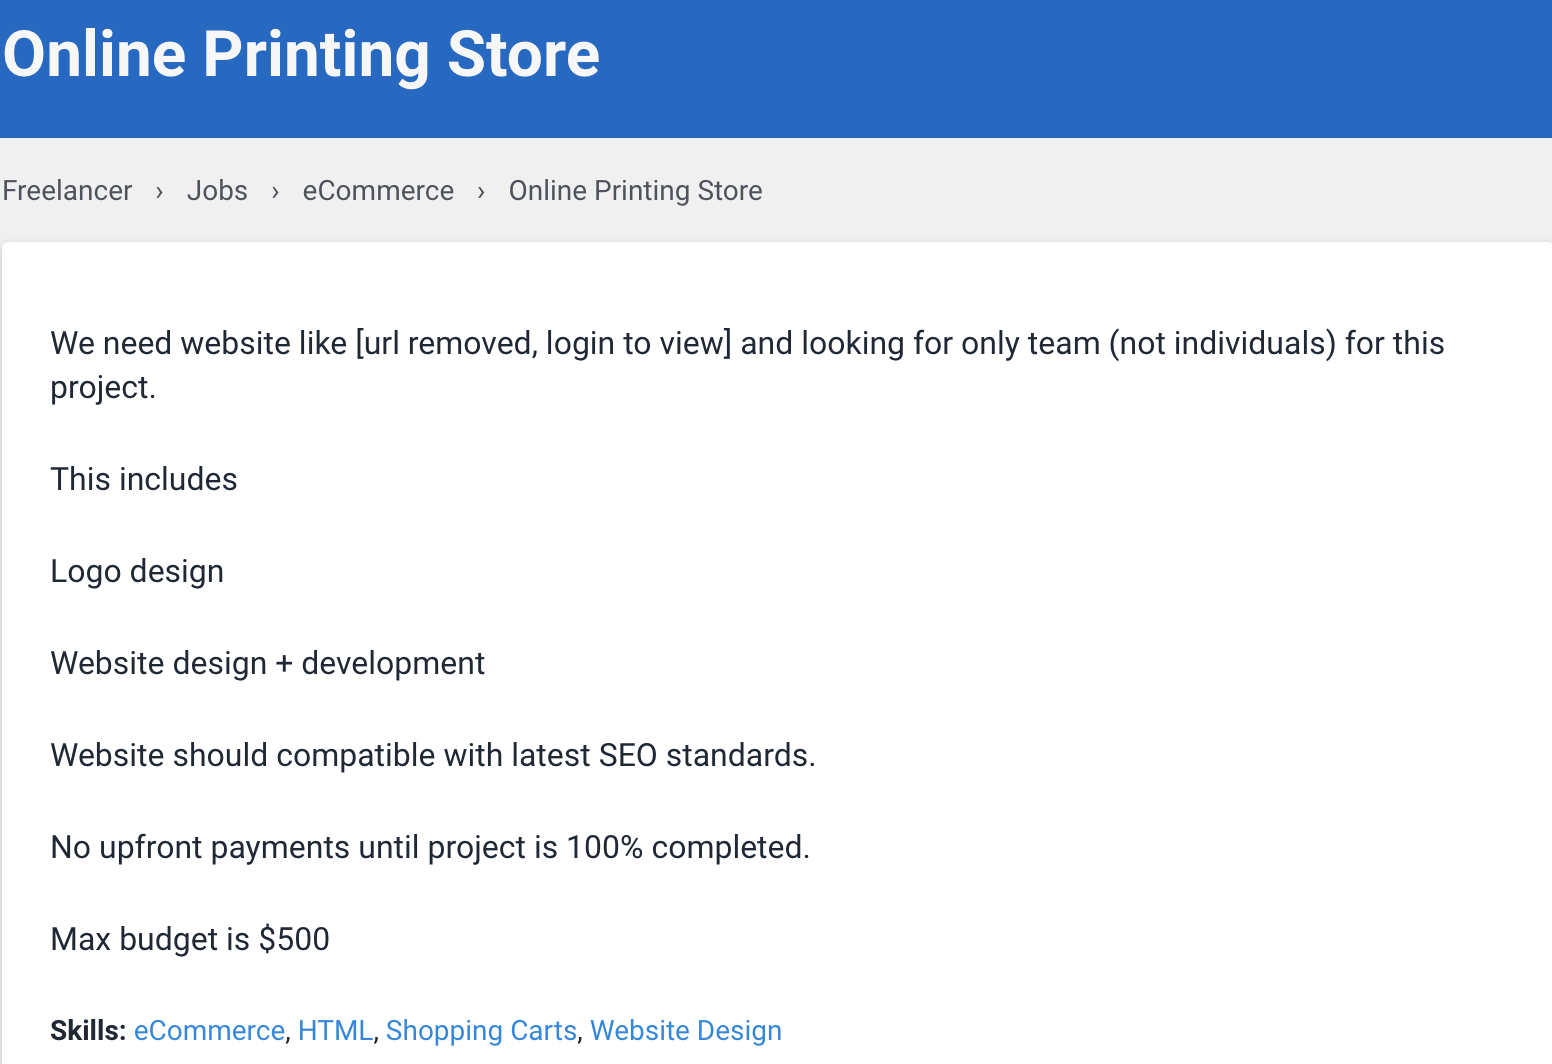
\includegraphics[width=\textwidth]{figures/FreelancerExample.png}
	\caption{An example project from the Freelancer Website}
	\label{fig:freelancer-example-project}
\end{figure}


As you can see in the figure \ref{fig:freelancer-example-project}, a typical freelancer project posting consists of a title, the description and the relevant skills. For simplicity, the thesis at hand only concentrates on the skills and doesn't take the project description into account. This would be topic of another paper/thesis, as it would require natural language processing and other techniques ~\parencite{bird2009natural}.


\begin{figure}[!ht]
	\centering
	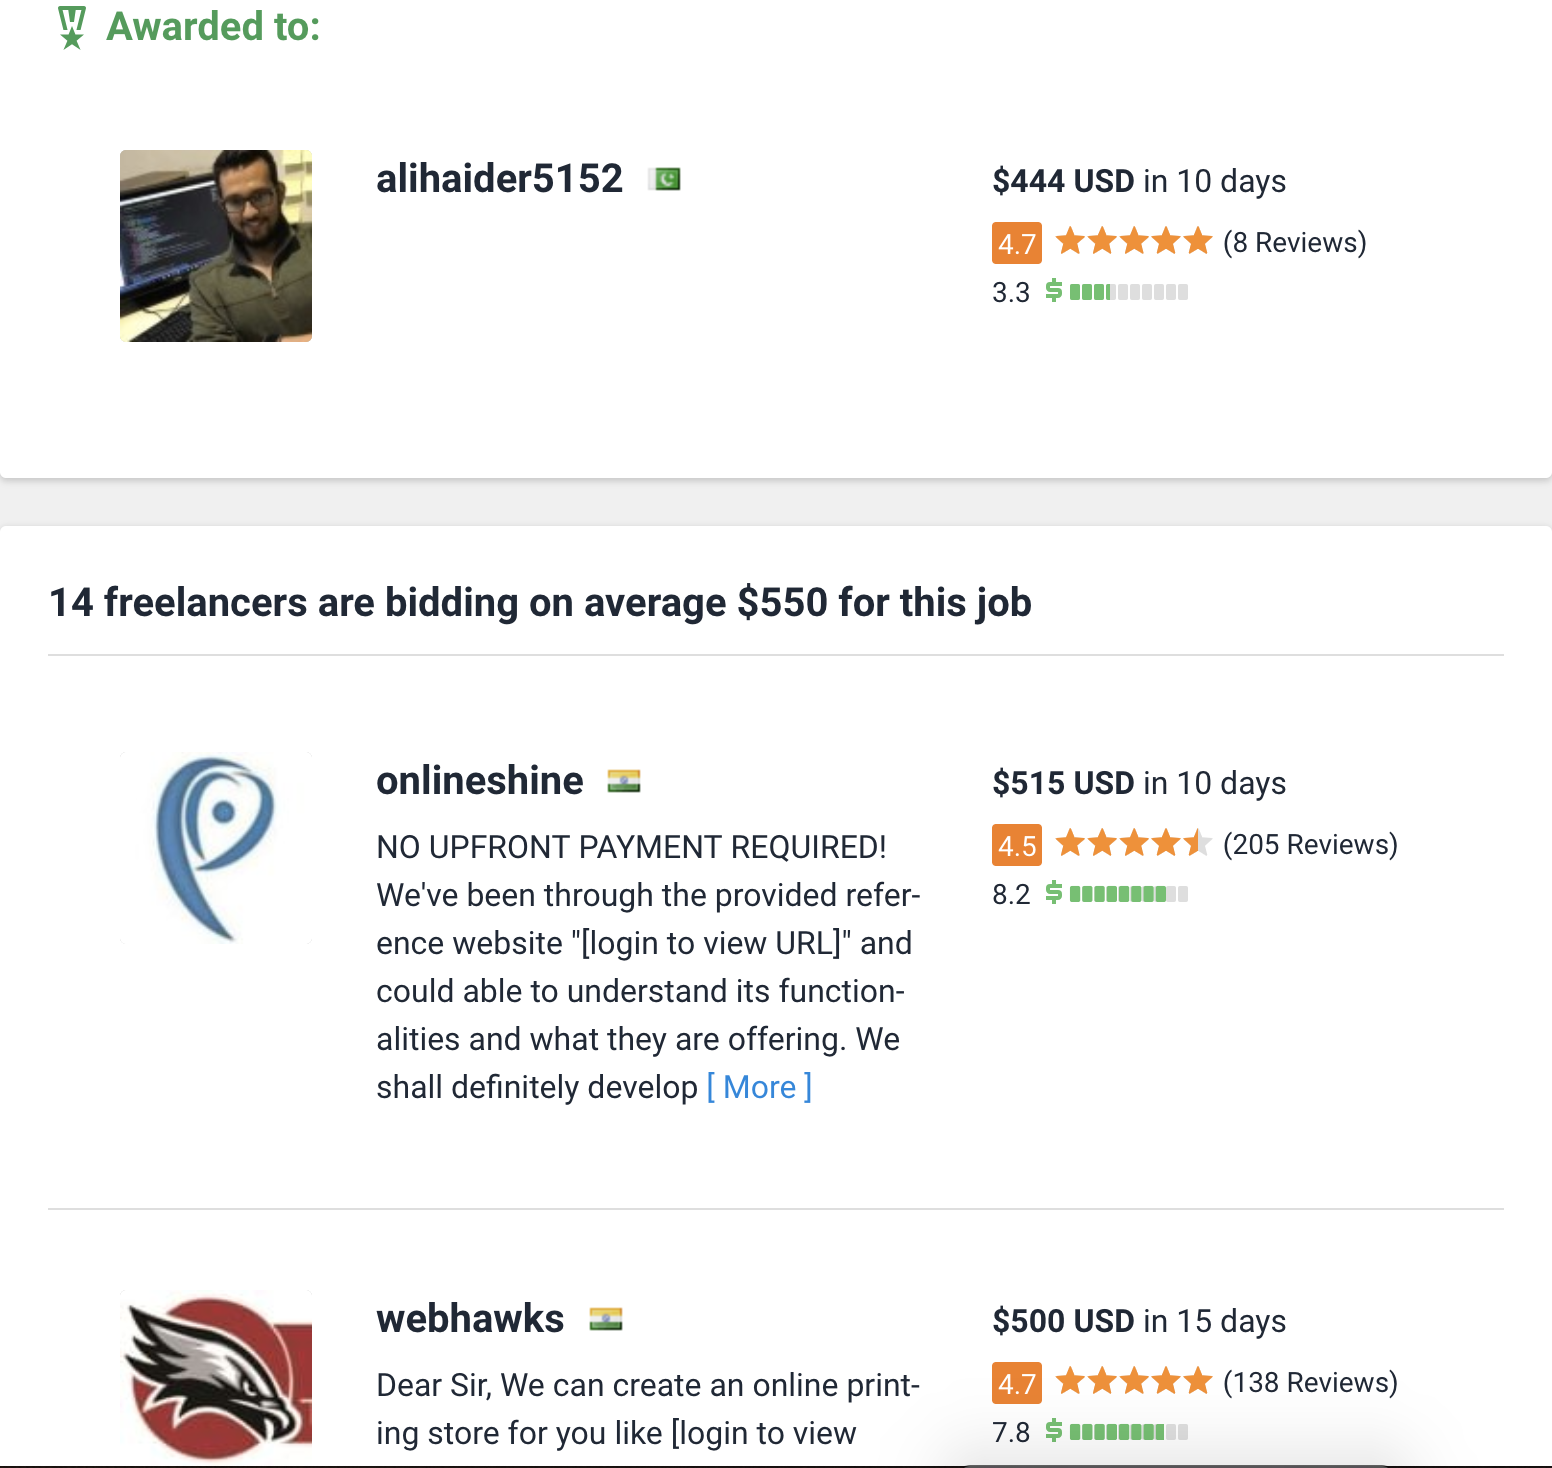
\includegraphics[width=0.75\textwidth]{figures/FreelancerTalentExample.png}
	\caption{The winner and other bidders to the same project}
	\label{fig:freelancer-example-talent}
\end{figure}


The figure \ref{fig:freelancer-example-talent} shows the bidders of the same project as above. The first one of the bidders has won the bidding race, which is decided by the creator of the project. The bidders include information such as a motivation text, the demanded monetary amount, their star rating until the time of bidding, amount of reviews they received and their total earnings until that date. In this thesis, we only consider the money they demand, their star rating and the number of reviews. For the sake of simplicity, we don't use the motivation text.


Each bidder lists their skills on their profile page and the employers may check their profiles before hiring talents. The figure depicts top skills of an example talent, which are listed in a descending order. The number near each skill shows how many related projects the talent completed. That's why the numbers can range from one to more than hundreds. 


\begin{figure}[!ht]
	\centering
	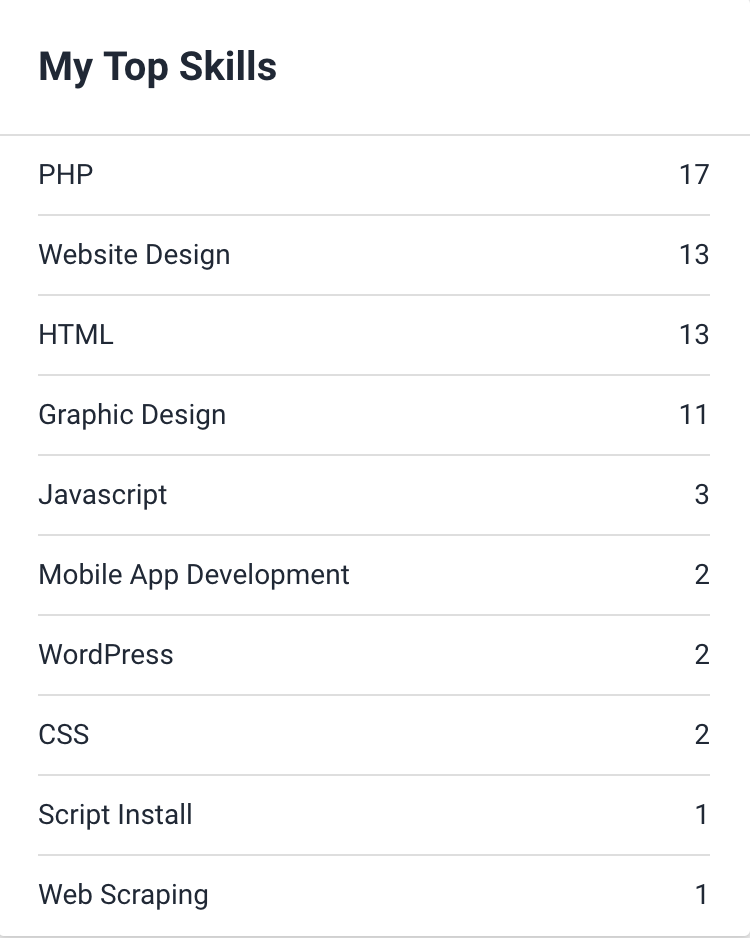
\includegraphics[width=0.5\textwidth]{figures/FreelancerTalentSkills.png}
	\caption{The list of tops skills by a talent on Freelancer web page}
	\label{fig:freelancer-talent-talent}
\end{figure}


The dataset encloses  941 unique skills, which are both technical and non-technical. However, the author of the thesis chose to limit these skills to 780, since some of them weren't used in notable amounts and the data can be expressed without using those skills. [TODO see dimensionality reduction add to research]


This dataset was scraped from freelancer.com by Philip Offtermatt, who also took part in this very project.


\subsection{Company Dataset}\label{subsection:company-dataset}

The company dataset at hand is acquired from the sponsor of this thesis, which is Motius GmbH. This dataset exported from their internal database and contains information of 795 people and 375 roles. Each role contains the required skills for the role and each person has their skills listed. One difference to the freelancer dataset would be that the talents also include skills that are associated with their original skill set. In theory, this is called association rules and the skills that are mostly used together are considered to have a correlation score of 1. Because of these correlations, each talent has many skills listed, some of them highly correlated and others are not correlated at all.


The amount of unique skills in the company data equals to 1768. Nonetheless, more than 85\% of the skills are used rarely, so the author reduced the unique set of skills to  202. Both of the datasets combined, there are 923 unique skills that were given at least 5 times. A problem we have with the datasets are the naming. Since, both Freelancer and Motius have used different names for skills, there are exists only a set of 59 common skills. Therefore, training both datasets together doesn't improve model like it's expected[TODO: evaluation neural network 10 000 data training falan filan].


When all of freelancer and company dataset are put together in their raw form, the matrix that contains all talent and project data reaches the size of 8 GB. This created a big problem for the author of the thesis. Since we only had available physical memory of 16 GB, working with an 8 GB matrix wasn't possible. When an operation like normalization is being done, the library \textit{Pandas} applies many copying operations, which doubles the memory usage and crashes. That's why the author employed embeddings as a dimensionality reduction mechanism[See \ref{subsection:using-embeddings}].



\section{Unsupervised Individual Recommender}

\subsection{Recommendation by Similarity}

As it was mentioned before, the unsupervised learning techniques focus on  learning without use of labels. Therefore, in the context of this thesis, we find similarites between projects and talents by using their feature vectors. 


\begin{equation}
\cos (x, y)=\frac{(x \bullet y)}{\|x\|\|y\|}
\end{equation}


The similarity measure we use for this part of the thesis is the cosine similarity ~\parencite{amatriain2011data}. The formula for the cosine similarity is shown above. The inputs  \textit{x and y} in the formula can correspond to a project-talent or a talent-talent pair. The types of input are document vectors of an n-dimensional space and the formula calculates the similarity as cosine of the angle between two vectors. The formula first calculates the dot product of the vectors and then divides it by the multiplication of the norm vectors.


To get the most relevant talents for the project, we calculate the cosine similarity between a selected project and every other talent. Then the algorithm sorts the talents by similarity and returns \textit{top n} talents.


\subsection{Recommendation by Popularity}


Another unsupervised recommendation mechanism that is used as a baseline is the popularity recommender. The popularity recommender is a hard to beat algorithm, that increases user satisfaction. [TODO add pages 394 and 395 to research section(from book)]]. The logic comes from the fact that, the \textit{items} that are in demand approved by many \textit{people}. That's why it's likely that selecting these items will increase the user satisfaction ~\parencite{amatriain2015recommender}. 


For this specific project, the popular items that are in demand are the people that finished the maximum amount of projects at Freelancer or at Motius. Although the results won't be personal, recommending the same successful talents is a nice strategy to acquire proven talents. The proof of this approach is shown in the subsection \ref{subsubsection:eval-popularity}.

\subsection{Hybrid Recommendation}

As a last submethod of unsupervised individual recommenders, we can name the hybrid recommender. Hybrid methods are also called as \textit{ensemble learning} methods. This technique combines the results from multiple methods and outputs a new result ~\parencite{beliakov2015aggregation}. For our use case, the author implemented different versions that combine the similarity recommender and the popularity  recommender. We can merge both of the recommenders by adding or multiplying the results. It is also possible to give different weights to these sources.


\section{Supervised Individual Recommender}\label{section:supervised}

Supervised learning means creating a model that learns with the help of labels. In our project, the author conceptualized labels as 0 or 1. 1 is for the case of the person got accepted for the project at freelaner.com or at Motius. 0 is for the case that the person got rejected. The models try to predict if the talent should be hired for the project or not(1 or 0).

For this task, we use two different versions; one version that takes all the skills as-is, the other one creates embeddings[TODO: embeddings in research chapter]. Both of the methods employ neural networks[TODO: neural networks in research chapter].


\subsection{Using Sparse Input}

\begin{figure}[!ht]
	\centering
	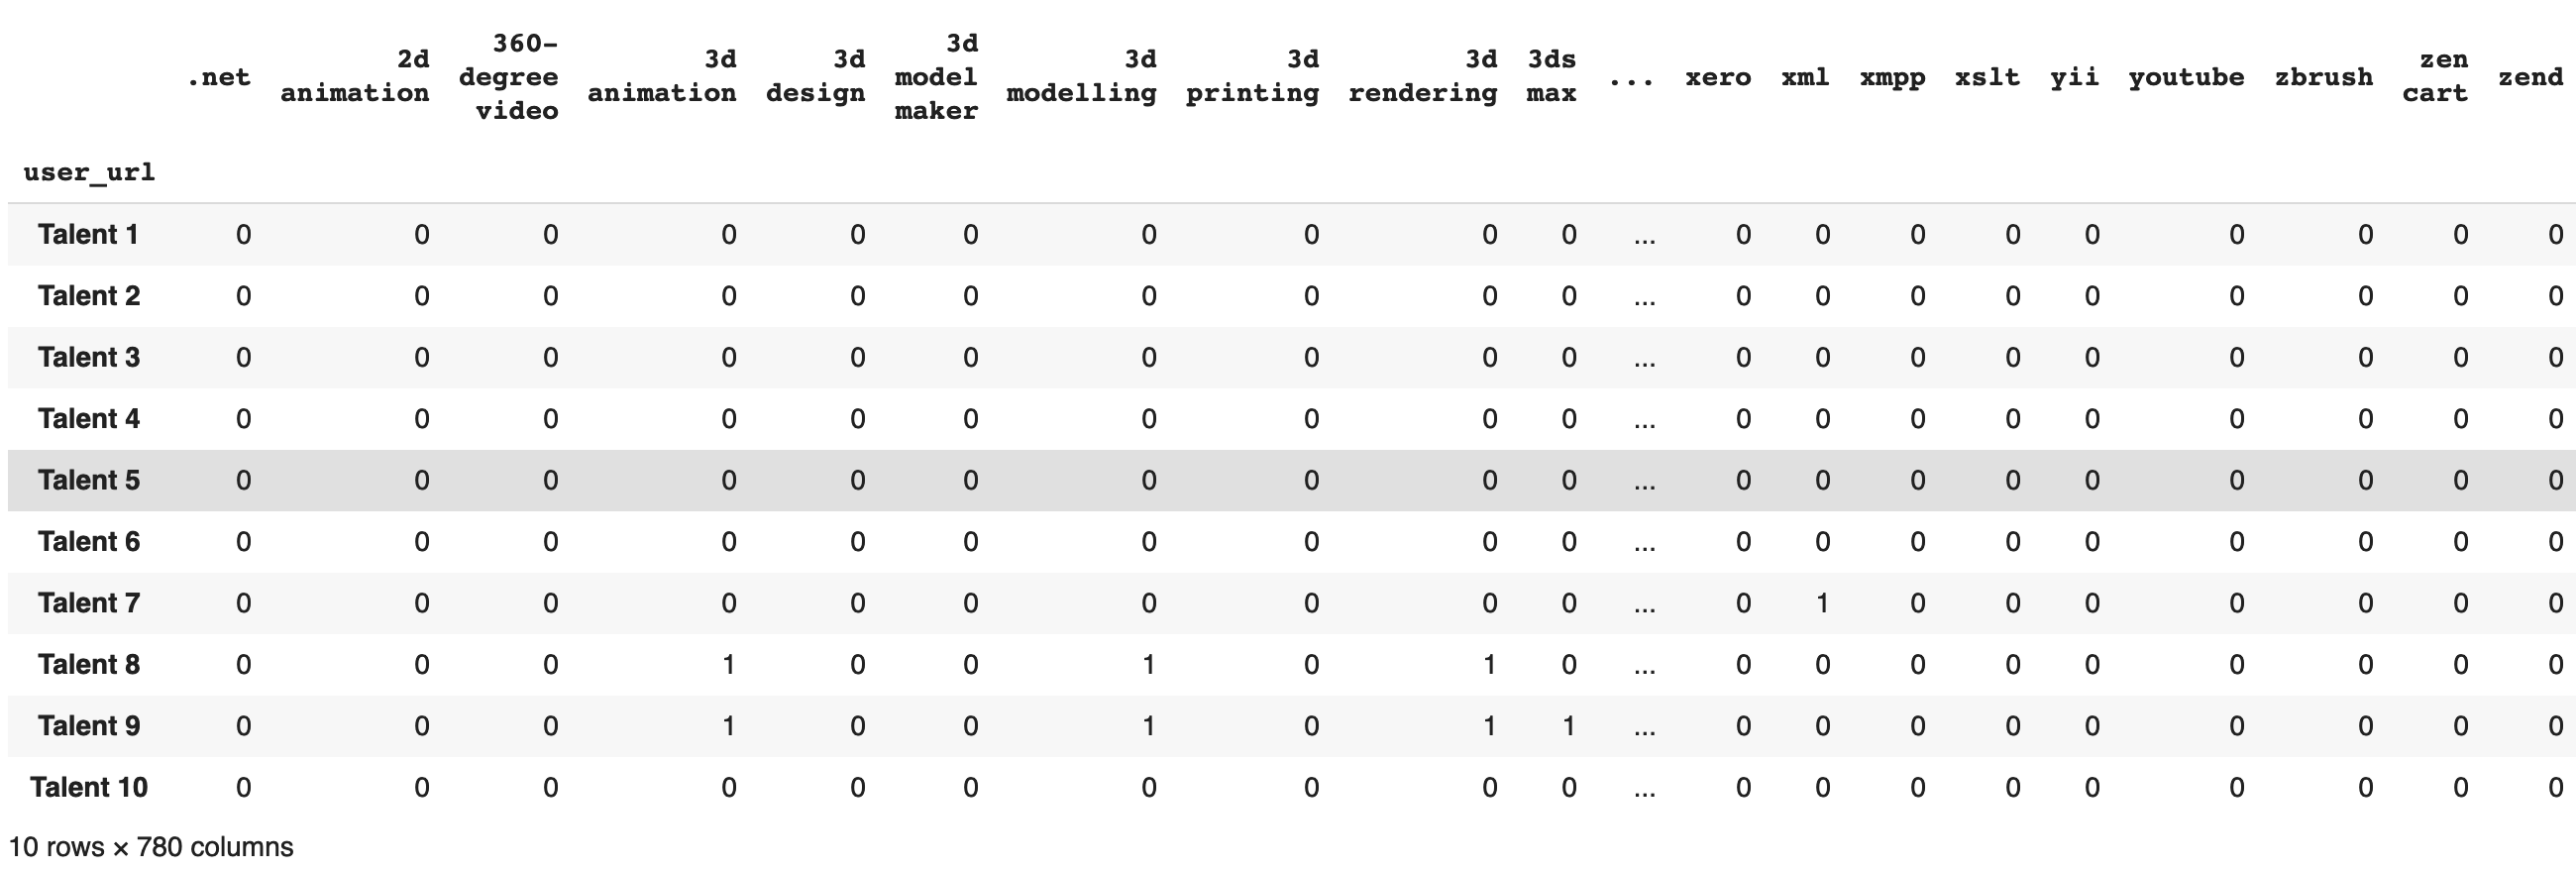
\includegraphics[width=\textwidth]{figures/FreelancerTalentSkillsMatrix.png}
	\caption{The talent skill matrix from freelancer.com}
	\label{fig:freelancer-talent-matrix}
\end{figure}

The first option that comes to mind is using the data as it is and training the model with them. The format of the talent data is shown on the figure \ref{fig:freelancer-talent-matrix} and the projects skills matrix also have the same format with project names as keys.

\begin{equation}
z = (x - u) / s
\label{eq:normal}
\end{equation}

According to experts ~\parencite{sola1997importance}, it is crucial to normalize input data before training neural networks. It has two significant benefits; it reduces the estimation errors and it cuts down the training time. That's why we normalize all of the inputs using \textit{StandardScaler} module of \textit{scikit-learn}. It uses equation \ref{eq:normal} to scale the data. In the equation, \textit{u} is the mean and \textit{s} is the standard deviation.

As it was mentioned before [See section \ref{section:datasets}], the freelancer.com dataset accommodates some extra information like experience level, star rating, number of reviews and hourly rate. These extra information of 10 example talents are shown in the figure \ref{fig:freelancer-talent-meta}. Since this information doesn't exist in Motius dataset, this subsection focuses only on the implementation with freelancer dataset. The extra information that is mentioned is also scaled and input into the neural network. 


After normalizing data, we prepare the matrix that is fed into the neural network row by row. For each bid in the freelancer data, we create a vector of length 1565. 780 of these values correspond to talent skills, the next 780 correspond to project skills, 4 of them are the extra information that are mentioned above and the last of them is for the outcome. Outcome is 1 for the case that the person received the project and 0 for the case that the person didn't receive the project.


\begin{figure}[!ht]
	\centering
	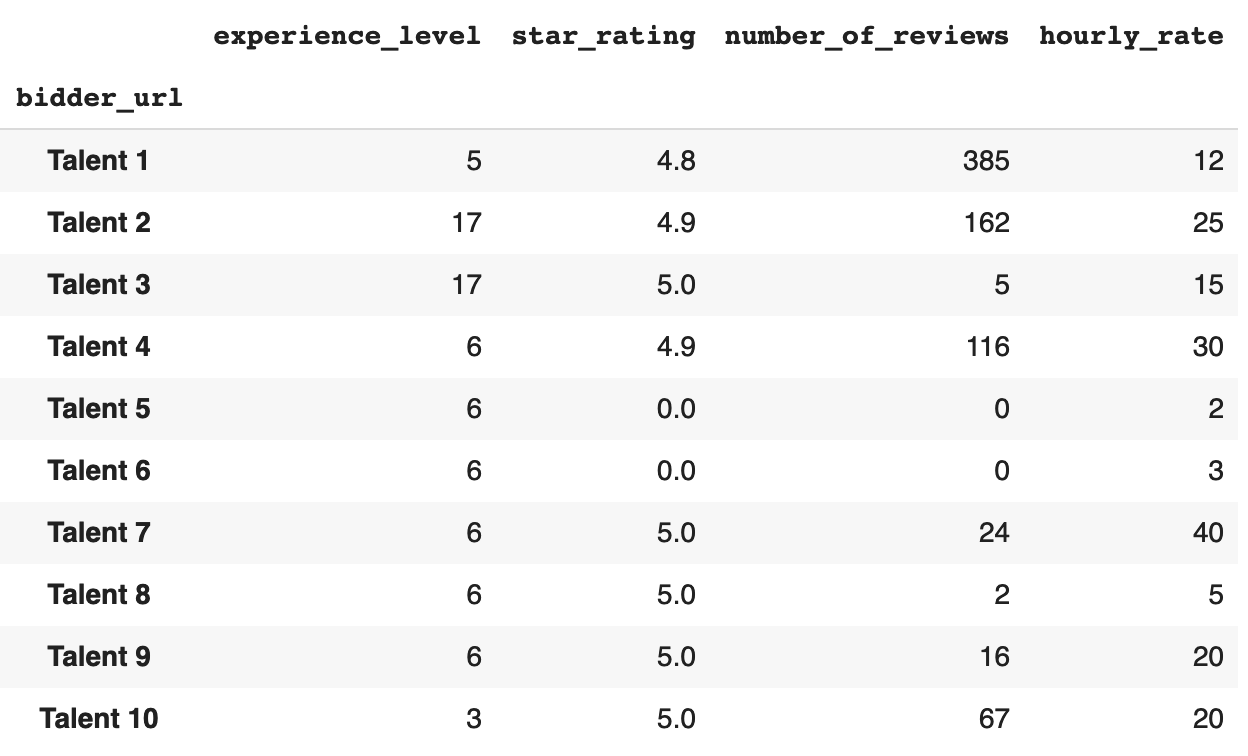
\includegraphics[width=0.75\textwidth]{figures/FreelancerTalentMeta.png}
	\caption{The talent extra information matrix from freelancer.com}
	\label{fig:freelancer-talent-meta}
\end{figure}

As one would expect, the model tries to guess if the person should be employed or not. Out of the \textit{321225} data points in total, we use 60\% for training, 20\% for test and the rest for validation. We split the data into those sets randomly using \textit{train\_test\_split} function of \textit{scikit-learn}. An important parameter not to miss is \textit{stratify}; since our dataset has  6\% positive and 94\% negative samples, we need to make sure that the this ratio remains also in the sets. Not using this feature could result in the model always predicting the same negative results. This means that the model would learn the same result, no matter what ~\parencite{singh2015survey}.

After splitting the data, we can start with training. There exists also some important features that we need to use; these optional features all have different objectives but they all serve to improve the results. These features are all supported by the packages \textit{Keras} and \textit{TensorFlow}, which are open-source neural network libraries. Keras is an abstraction layer for TensorFlow that lets the users to train neural networks with minimal number of lines ~\parencite{chollet2018deep}. While fitting the model with training data, Keras gives the option to add callbacks. The callbacks that we adopt are \textit{EarlyStopping}, \textit{ModelCheckpoint},  \textit{ReduceLROnPlateau} and \textit{TensorBoard} . As the name suggests, early stopping [TODO: add neural networks to research part, also validation loss, overfitting, graph vs] serves to prevent overfitting. In our case, it compares the validation loss of current batch with the previous one. If the validation loss doesn't drop for 10 times, the training stops. The next callback model checkpoint is used complementary to early stopping. Model checkpoint saves the model weights of the batch with the minimum validation loss. After the training is done, we load those model weights that achieved the best accuracy. ReduceLROnPlateau reduces learning rate when the validation loss has stopped improving. Lastly, TensorBoard is a visualization tool of TensorFlow. It produces model visions and graphs that show the evolution of the accuracy, loss and learning rate. 

When we are training the model, we should also set the training weights for both labels manually. The dataset encompasses 6\% positive and 94\% negative samples, so we need to penalize the errors according to this rate. After training, the class weights are ignored and not used in testing/predicting.


The figure \ref{fig:tensor-board-sparse}  depicts the model that is used to predict if a talent should be employed or not. The direction of the graph starts at the bottom of the image and goes up. Like it was mentioned before, the model expects three feature vectors. These vectors are defined as the skill vectore of the project, the skill vector of the talent and extra information of the talent(e.g. hourly rate, total experience). 

 \begin{figure}[!ht]
	\centering
	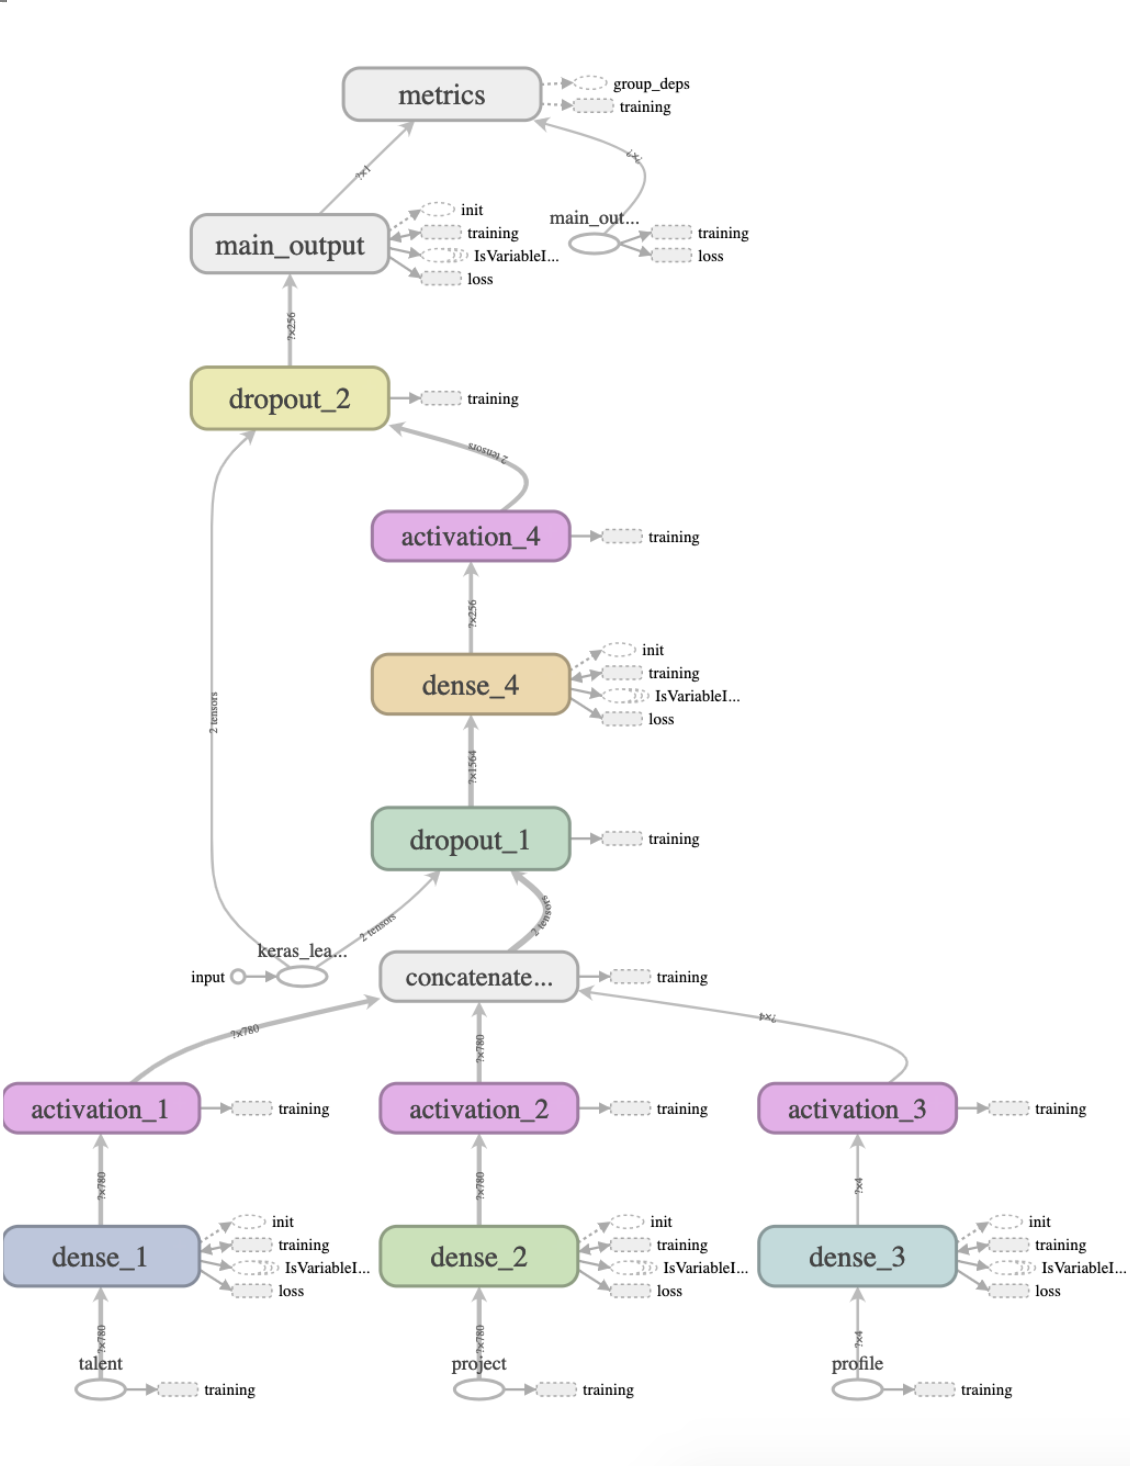
\includegraphics[width=0.75\textwidth]{figures/TensorBoardSparseCropped.png}
	\caption{The graph that explains the sparse input model}
	\label{fig:tensor-board-sparse}
\end{figure}

For each of the inputs, a dense layer exists with number of neurons equal to number of features. This means that project and talent layers contain 780 neurons and profile information layer contains 4 neurons. For these layers, we use \textit{relu} activation, \textit{l1} regularization with the value \textit{0.0001} and we initialize the weights with \textit{he normal}. Detailed knowledge about activation, regularization and weight initialization can be found in the ~\autoref{chapter:review_of_research}[TODO: add activation, regularization and weight init to research chapter].



After the activation functions, all layers get concatenated horizontally. This is followed by a dropout layer with half of the neurons are disabled randomly[TODO: add dropout to neural networks section of chapter 2]. Next one in the model is a dense layer with 256 nodes, which possesses the same activation function, regularization and weight initialization methods as the previous dense layers. The model accommodates a last dropout layer and ends with the main output. The output is only a one node layer and involves a \textit{sigmoid} activation function that squeezes the output value to be between 0 and 1[TODO: research -> nn -> activation functions -> sigmoid]. The weight initializer of the last layer is \textit{glorot uniform}.[TODO: research -> nn -> weight initializers -> glorot uniform].

\begin{equation}
C(w, b) \equiv \frac{1}{2 n} \sum_{x}\|y(x)-a\|^{2}
\label{eq:mean-squared-error}
\end{equation}

Each neural network has the aim of minimizing their cost function ~\parencite{Goodfellow-et-al-2016}. The cost function that we chose is \textit{mean squared error}[See ~\autoref{eq:mean-squared-error}]. This example of cost function is used mostly for regression tasks and calculates the mean squared difference of the actual value and the predicted output value. The metric we use is accuracy and more information about it can be found in ~\autoref{chapter:evaluation}.


\subsection{Using Embeddings}\label{subsection:using-embeddings}

High-dimensional spaces and distributions  prove to be unexpected and completely differ from low-dimensional spaces. The empty space phenomenon and other ones are examples of the \textit{curse of dimensionality}. With the help of embeddings layers, we can represent high-dimensional data in low-dimensions  ~\parencite{lee2007nonlinear}.

Although deep neural networks have the ability to avoid the  curse of dimensionality ~\parencite{poggio2017and}, we still need to use embeddings layers for spatial reasons. In the previous sections, we mentioned that there are 780 unique skills for freelancer data and 923 skills if we also add Motius data. This means that the data has 923 dimensions and we know that the data is sparse, most of the data matrices consist of zeroes, so we can actually reduce the dimensionality. 

[TODO explain embeddings and move this image to research. also explain embeddings math. instead, put the actual embedding image here from TensorBoard]
 \begin{figure}[!ht]
	\centering
	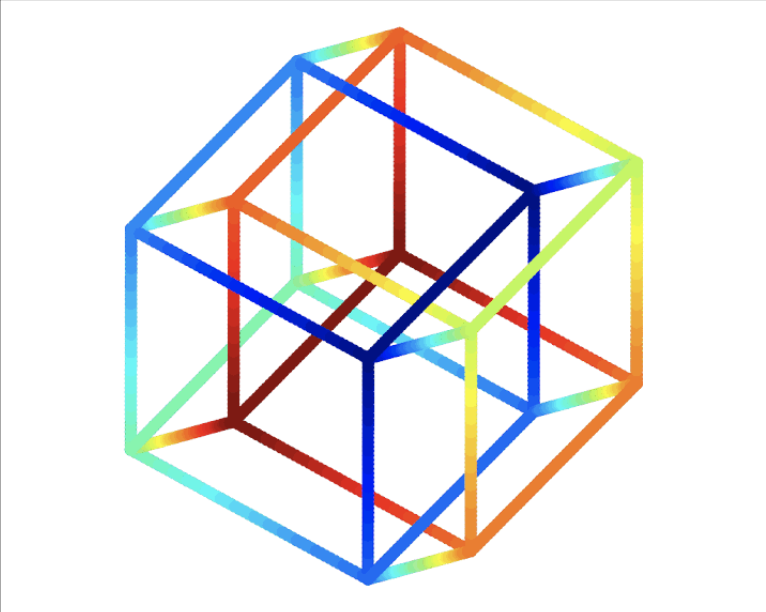
\includegraphics[width=0.75\textwidth]{figures/DimensionalityReduction.png}
	\caption{2D representation of a 4D cube. The colors indicate the depth in fourth dimension ~\parencite{lee2007nonlinear}.}
	\label{fig:embedding-projection}
\end{figure}


\subsubsection{Preprocessing}

For both Freelancer and Motius data, we know the skill levels of projects and talents for various of skills. Instead of having some positive and hundreds of zero skill values for each project/talent, we can set a skill threshold. This threshold implies skills above or equals to the threshold are positive and the rest are zero. The idea is converting the talent-skill and project-skill matrices so that, each talent/skill holds list of skills they know/require. However, another constraint that need to be addressed is the maximum length of the padded skill matrix, because neural networks require a fixed input shape. Therefore, the talent/project maximum amount of positive skills is determined. For Freelancer data, this is 18, which means all skills vectors are padded with zeroes to have the length of 18. 

In the case of Motius data, the topic is more complex. The ~\autoref{subsection:company-dataset} explained how the correlation mechanism of the company data works. To explain it briefly, Motius stores user skills and other skills that are correlated for each user. This has the effect that there exists many skills for each user but most of these skill levels are low. Here the highest skill level would 2 and lowest would be 0.

\begin{figure}[htpb]
	\centering
	
	\pgfplotstableset{col sep=&, row sep=\\}
	% This should probably go into a file in data/
	\pgfplotstableread{
		a & b    \\
		0.1 & 780 \\
		0.2 & 732 \\
		0.3 & 676 \\
		0.4 & 605 \\
		0.5 & 530 \\
		0.6 & 463 \\
		0.7 & 386 \\
		0.75 & 361 \\
		0.8 & 325 \\
		0.9 & 299 \\
		1.0 & 269 \\
	}\exampleA
	\pgfplotstableread{
		a & b    \\
		0.1 & 132 \\
		0.2 & 112 \\
		0.3 & 94 \\
		0.4 & 71 \\
		0.5 & 57 \\
		0.6 & 44 \\
		0.7 & 28 \\
		0.75 & 21 \\
		0.8 & 16 \\
		0.9 & 12 \\
		1.0 & 9 \\
	}\exampleB
	% This should probably go into a file in figures/
	\begin{tikzpicture}
	\begin{axis}[
	ymin=0,
	legend style={legend pos=outer north east},
	grid,
	thick,
	ylabel=Threshold,
	xlabel=Amount
	]
	\addplot table[x=a, y=b]{\exampleA};
	\addlegendentry{Amount of Motius talents};
	\addplot table[x=a, y=b]{\exampleB};
	\addlegendentry{Maximum skill vector length};
	\end{axis}
	\end{tikzpicture}
	\caption[Threshold figure]{Effect of threshold selection on talents and maximum skill vector length}\label{fig:threshold-selection}
\end{figure}

The effect of different threshold values on Motius data is shown on \autoref{fig:threshold-selection}. Without any threshold, there is a couple of Motius projects with the maximum skill length of 21. Projects don't specify skill levels so these are taken as they are. That's why, we also wanted to have a similar maximum length for Motius talents. When there is no threshold, there are 780 Motius talents with at least one skill value but the maximum skill vector length is 132. We wouldn't want to implement this version because the maximum length of 132 will create millions of zeroes in the dataset, which we wanted to avoid in the first place. Setting the threshold to a high value(like 1 or more) is also not optimal, since it limits the maximum skill vector length to 9 and number of Motius talents to 269. Having such a high value would decrease the amount of informatio we have significantly,  because the Freelancer data also has a maximum length of 18. Therefore, the optimum threshold value we reached is \textit{0.75}. Doing this, limits the number of Motius talents to 361 and limits the maximum skill vector length to 21, just like the project with the most skills.

\autoref{fig:embedding-training-matrix} depicts the training data with padded skill matrix. The columns with the numbers in range 0 to 20 are the indices of the talent skills. The columns with the numbers 21 to 41 are project skills indices.  The version of the image is the one with the Motius and Freelancer data combined. In the variant with only Freelancer data, we have skill vector lengths of 18 and the extra information of talents included.

 \begin{figure}[!ht]
	\centering
	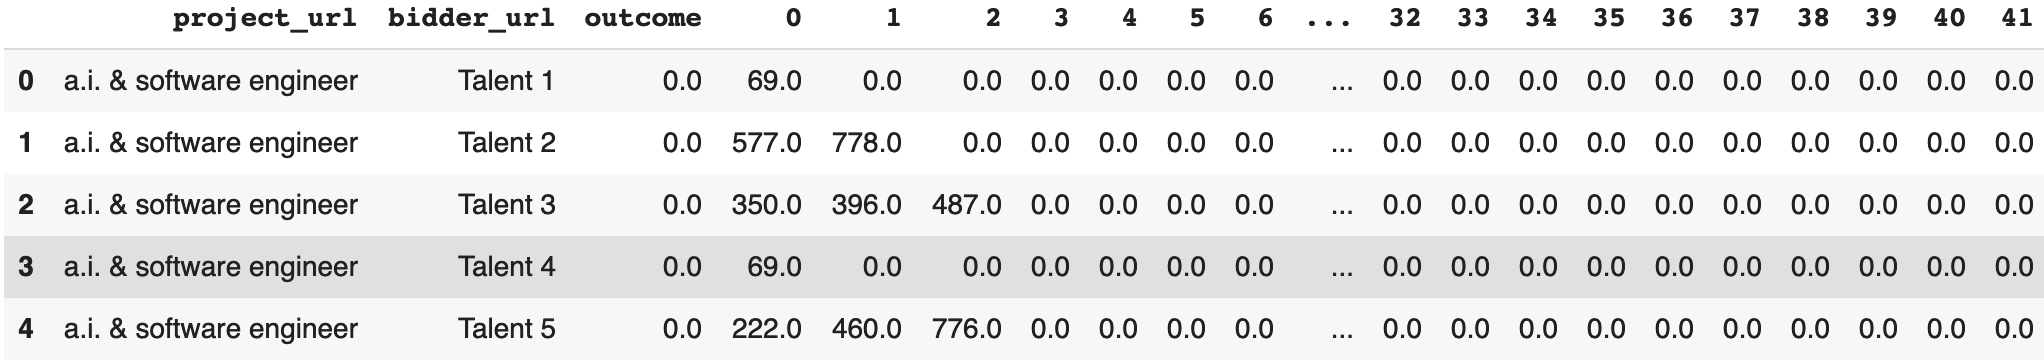
\includegraphics[width=\textwidth]{figures/EmbeddingTrainingMatrix.png}
	\caption{Training data that contains padded embedding skill vectors}
	\label{fig:embedding-training-matrix}
\end{figure}



\subsubsection{Simpler Architecture for Company Dataset}

The Freelancer dataset has a huge advantage over Motius data, which is the extra information that we know about the applicants. When we use both datasets together to train a model, we can limit the inputs to talent and project skills. 

\autoref{fig:model-code} illustrates the simplified version of the \textit{Python} code that constructs the model to predict the hiring result. The \textit{features} parameter of the model building function corresponds to the length of padded skill vector and the next parameter \textit{dimensions} represents total amount of unique skills. Embedding layers in Keras expect the arguments \textit{input dimension}, \textit{output dimension}, \textit{input length} and the optional flag \textit{mask zero}. As embeddings only accept positive integers, input dimension should be the size of the vocabulary, which is number of total skills in the recommender system. The value of the output dimension can be decided by the developer and explains the size of the desired output dimension. Although, there is no scientific document that states an ideal output dimension, trial-and-error method showed that the best result is achieved with the fourth root of the number of dimensions. The additions of one in multiple places in code are due to using the mask zero operation. Zeros in rows get filtered out, which increases the performance and speeds up the training process. The cost function that we use is \textit{binary crossentropy}, because we want to optimize the process of hiring or not hiring a talent to the project. [TODO: research -> cost functions -> binary crossentropy]. Lastly, \textit{sigmoid} activation function squeezes the output value to be between 0 and 1[TODO: research -> nn -> activation functions -> sigmoid].



\begin{figure}[!ht]
	\centering
	\begin{tabular}{c}
		\begin{lstlisting}[language=Python]
		def nn_embedding(features, dimensions):
		  talent = Input(shape = (features,))
		  project = Input(shape = (features,))
		  output_dim = int(dimensions ** 0.25) + 1
		
		  talent_embedding = Embedding(dimensions + 1, output_dim,
		  input_length=features, mask_zero=True )(talent)
		  project_embedding = Embedding(dimensions + 1, output_dim,
		  input_length=features, mask_zero=True)(project)
		
		  # these are required because of mask zero
		  talent_embedding = Lambda(lambda x: x,
		  output_shape=lambda s:s)(talent_embedding)
		  project_embedding = Lambda(lambda x: x,
		  output_shape=lambda s:s)(project_embedding)
		
		  merged = Concatenate()([talent_embedding, project_embedding])
		  merged = Flatten()(merged)
		  merged = Dropout(0.5)(merged)
		  main_output = Dense(1, activation='sigmoid')(merged)
		
		  model = Model(inputs=[talent, project], outputs=[main_output])
		  model.compile(optimizer='adam', loss='binary_crossentropy',
		  metrics=["accuracy"])
		
		  return model
		\end{lstlisting}
	\end{tabular}
	\caption[Model Code]{The code of the model for both Motius and Freelancer data}\label{fig:model-code}
\end{figure}

\section{Unsupervised Group Recommender}\label{section:unsupervised-group-rec}

In this section, we explain the process of recommending multiple talents to super groups. The methods that are used for this part are derivations of the ones that are used in individual recommenders. Therefore, the basic concepts that are used before also apply here. 

To perform group recommendations, projec-role or project-project information are needed. The website freelancer.com shows other projects from the same supervisor, which can be combined. Then these projects will form a superproject and projects can be treated as roles of a bigger project. For Motius data, we already possess this information as project-role data. Roles of Motius correspond to the projects in the Freelancer data. In terms of simplicity and shortness, we only take Freelancer dataset with groups of size 5 into account. 

\subsection{Baseline}

The basic appoach to unsupervised group recommendations would be calculating the cosine similarity between each project and talents. Then picking the best talents and listing them. However, the results won't be diverse and we can pick talents that have similar skills to each other. We want to avoid that [TODO add different evaluations to both theory and their results to evaluation part!] and have diverse recommendations for each project.

\subsection{Diverse}

Because of the reasons above, we want to create the recommendation list in a diverse way from the beginning. The topic of diversity is already explained before[TODO: reserach -> diversity enhancement] and the pseudocode to enhance diversity is shown below.

\begin{equation}
\begin{array} { l } { R \leftarrow \emptyset } \\ {  while\, | R | < k\,: } \\ { \quad i * \leftarrow \arg \max _ { i \in C - R } g ( R \cup \{ i \} , \lambda ) } \\ { \quad R \leftarrow R \cup \{ i * \} } \\ { end\, while\,  } \\ {  return\,  R } \end{array}
\label{eq:diversity-enhancement}
\end{equation}


In the algorithm above, we first create an empty recommendation list \textit{R} and set a recommendation length \textit{k}. In our example, we only consider the groups with project amount of 5, so \textit{k} is 5 as well. After that, we find the the optimal candidate that hasn't been selected yet, is relevant to the project at hand and is also diverse to the other selected candidates. Finding the optimal candidate can be tuned with the help of \autoref{eq:diversity-equation}. The $\lambda$ parameter in the equation can be tuned to value the relevancy or diversity more; $\lambda$ of 1 means to only consider diversity, 0 means to only consider relevancy and 0.5 gives the balanced result. When we receive the optimal candidate from the equation, we add them to the recommendation list and iterate until we have enough talents for the whole group.

\begin{equation}
g ( R , \lambda ) = ( 1 - \lambda ) \frac { 1 } { | R | } \sum _ { i \in R } f _ { r e l } ( i ) + \lambda d i v ( R )
\label{eq:diversity-equation}
\end{equation}

When we compare the diversity of the baseline approach to the diverse group recommendation, it is obvious that the diversity of talents recommended has increased. The evaluation algorithm for diversity and other relevant measures can be found in \autoref{chapter:evaluation}. [TODO group-rec evaluation]

\section{Supervised Group Recommender}\label{section:supervised-group-rec}

The previous section was about performing group recommendations with unsupervised learning. This section will do the same job using supervised learning model that we used in \autoref{section:supervised}.

\autoref{eq:diversity-equation} includes a $f _ { r e l } $, which is a relevancy score and a diversity rate that can be computed via cosine similarity, neural networks or other methods. In contrast to the unsupervised method, we calculate the relevancy score using the neural network that we used in \autoref{section:supervised}.

What we do in the individual supervised learning part is, training all parameters jointly, which is called end-to-end learning. This ideal was also the first aim for supervised group recommender approach. However, the data for such learning doesn't exist. To apply it, we would need data of hiring decisions for the groups not just projects. Since we don't have such information, we would have to generate it with a seperate algorithm. In the end, it wouldn't bring much, because the model would learn the data generation algorithm and wouldn't have an effect on the real-life hiring prediction.

Due to the reason above, step by step  learning process practiced. The first step of the process is training the model to optimize the individual hiring of talents. Then, we predict the relevancy score for each project-talent pair. For diversity score, we use the cosine similarity between the talents. After set those functions, the algorithm \ref{eq:diversity-enhancement} is applied.

In the end, this method increases diversity according to the evaluation methods that are listed in \autoref{chapter:evaluation}.

\subsection{Using Clustering}

Clustering is the process of dividing data into different groups. To perfom diverse multi-project recommendations, we can pick talents from clusters. Therefore, we can be sure that they are dissimilar. 

Since k-means clustering can suffer from the curse of dimensionality~\parencite{steinbach2004challenges} [TODO reseache: curse of dim, clustering ve k-means, pca ekle], To prevent it, it is logical to reduce the dimensionality first. The choice of the author to reduce dimensionality is \textit{Principal Component Analysis}.

The central idea of principal component analysis (PCA) is to reduce the
dimensionality of a data set consisting of a large number of interrelated
variables, while retaining as much as possible of the variation present in
the data set. This is achieved by transforming to a new set of variables,
the principal components (PCs), which are uncorrelated, and which are
ordered so that the first few retain most of the variation present in all of
the original variables~\parencite{jolliffe2011principal}. 

 \begin{figure}[!ht]
	\centering
	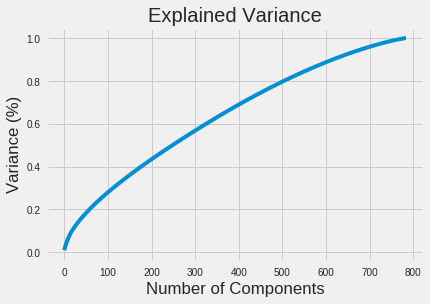
\includegraphics[width=0.75\textwidth]{figures/PCAExplainedVariance.png}
	\caption{Explained variance ratio for difference number of PCs is shown.}
	\label{fig:pca-explained-variance}
\end{figure}

To determine the number of PCs, the explained variance ratio for different amount of PCs can be checked. \autoref{fig:pca-explained-variance} shows how much of variance information we lose if we set the number of components to a certain value. Here, it makes sense to note that a higher number will the clustering model negatively and a lower number won't be able to capture everything in the dataset. The author of the thesis, experimented with different values.

\begin{equation}
a(i)=\frac{1}{\left|C_{i}\right|-1} \sum_{j \in C_{i}, i \neq j} d(i, j)
\label{eq:silhouette-a}
\end{equation}

\begin{equation}
b(i)=\min _{i \neq j} \frac{1}{\left|C_{j}\right|} \sum_{j \in C_{j}} d(i, j)
\label{eq:silhouette-b}
\end{equation}

\begin{equation}
s(i)=\frac{b(i)-a(i)}{\max \{a(i), b(i)\}}
\label{eq:silhouette-c}
\end{equation}

K-means clustering  requires a \textit{k} value that determines the number of clusters the model is going to create. The ideal number of clusters can be verified by calculating the silhouette scores for different number of clusters. The figure \ref{fig:pca-silhouette} shows silhouette scores for different cluster amounts. Silhouette score calculates how similar a data point to its own cluster compared to other clusters \parencite{rousseeuw1987silhouettes}. For this task, we use the equation in the equations \ref{eq:silhouette-a}, \ref{eq:silhouette-b}, \ref{eq:silhouette-c}. In the equations, different distance metrics can be employed. The choice of the author is euclidian distance[TODO: distance metrics research].  The equation \ref{eq:silhouette-a} calculates mean intra-cluster distance for each sample and the next \ref{eq:silhouette-b} computes mean nearest-cluster distance for each sample, which means the distance between a sample and the nearest cluster that the sample is not a part of. The last function \ref{eq:silhouette-c} converts the results of the first two equations into silhouette coefficients. The mean of all silhouette coefficients from every sample gives the silhouette score for that \textit{k} value. Higher silhoutte scores sugges that the samples well matched to its own cluster and poorly matched to neighboring clusters. In the example of \ref{fig:pca-silhouette}, it makes sense to select a value like 30. To visualize results, the centers of the clusters are projected on a 2D space[See \ref{fig:kmeans-centers}]. The X axis of the graph is the maximum value in each cluster center coordinate and Y axis of the graph is the maximum value in each cluster center coordinate.

 \begin{figure}[!ht]
	\centering
	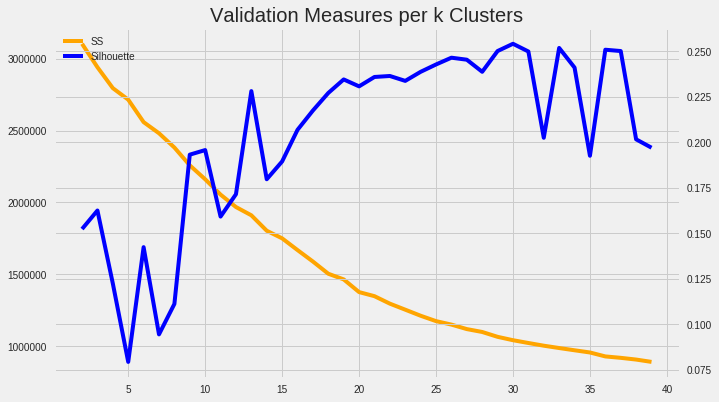
\includegraphics[width=\textwidth]{figures/PCASilhouette.png}
	\caption{Silhouette scores of many different \textit{k} values of k-means}
	\label{fig:pca-silhouette}
\end{figure}

Next, we benefit from another function of the PCA; \textit{inverse\_transform}. Inverse transform takes the cluster centers as an input and converts them to full talent values. This promises that we treat each cluster center like a talent and transform their values to skill values and extra information. In end, we possess an average skill vector for every cluster [See figure \ref{fig:cluster-centers-matrix}]. The figure contains some part of the skill vectors of the first three average talents. For example the cluster(segment) 0 in the figure has exceptional \textit{Adobe Illustrator} skills. Segment 1, on the other hand, is an all-rounder. Lastly, segment 3 is a \textit{c\#} developer.  It must be noted these values are calculated after standard scaling[TODO research -> standard scaling].

 \begin{figure}[!ht]
	\centering
	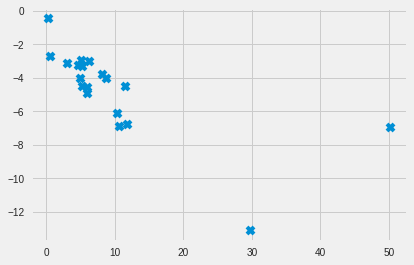
\includegraphics[width=0.75\textwidth]{figures/KMeansCenters.png}
	\caption{Centers of clusters that are projected on a 2D space}
	\label{fig:kmeans-centers}
\end{figure}



After we exercise clustering, we can start with group recommendation process. The recommendation can be operated both supervised[See \ref{section:supervised-group-rec}] or unsupervised[See figure \ref{section:unsupervised-group-rec}]. The same principles apply and we calculate relevancy score with cosine similarity or neural networks. In contrast to the other methods, the algorithm computes the relevancy score of the project and average cluster skills [See figure \ref{fig:cluster-centers-matrix}]. This way, we determine the ideal cluster for the project. When a project got recommended a talent from a specific cluster, that cluster is excluded from the next projects in the group. Therefore, a diversity in a group is guaranteed. After the selection of the optimal cluster, the best candidate in that cluster is chosen via neural networks or cosine similarity.

 \begin{figure}[!ht]
	\centering
	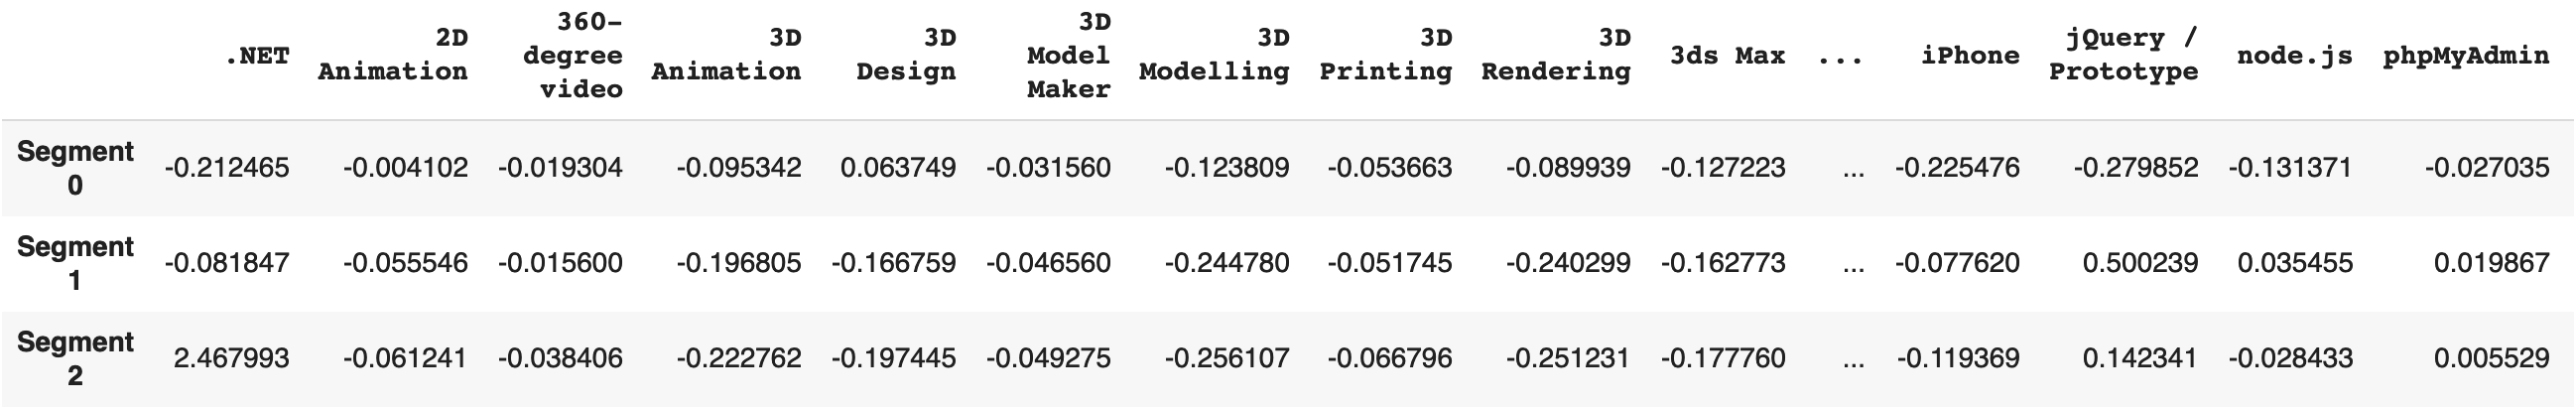
\includegraphics[width=\textwidth]{figures/ClusterCentersMatrix.png}
	\caption{Examples of some centers of clusters that are projected on a 2D space}
	\label{fig:cluster-centers-matrix}
\end{figure}



\section{Dashboard to show data and enter Feedback}

Another big part of the thesis is the dashboard that was built for various purposes; these purposes are showing individual unsupervised, supervised and hybrid recommendations for Motius and Freelancer datasets, showing group recommendetaions using unsupervised, supervised and hybrid methods and allowing to enter feedback, that have direct and indirect effects on the results.

The dashboard adopts the front-end that is programmed with \textit{Vue.js} and a back-end that employs \textit{Flask}[TODO: research -> frontend, backend, docker]. Vue.js is a front-end development framework that can be programmed with JavaScript. Flask is a back-end development framework that can be called with Python. The reason to use Vue.js is because of subjective reasons; it a reactive, modern framework that is easy to develop \cite{you2018vue}. Flask is on the other hand is chosen, because it is a popular leight-weight Python framework \cite{grinberg2018flask}. Since the rest of the machine learning training/prediction was done on Python, the author seized the opportunity to reuse/adapt the same codebase. 

Docker is a container virtualization technology, which like a very lightweight virtual machine. Adding Docker to our software stack gives the advantage of portability. This is important for various reasons; first of all the operating system choice of the author is \textit{MacOS} but most of the servers run different flavors of \textit{Linux}. All of the different operating systems have different installation methods, different pre-installed libraries and different dependencies. Docker solves this problem by standardizing the building and running operations of virtual machines. This way, the author was able to run everything on own computer and can be sure that it will also run perfectly on the servers of Motius if they choose to implement the solution on their internal system. \cite{anderson2015docker}.

 \begin{figure}[!ht]
	\centering
	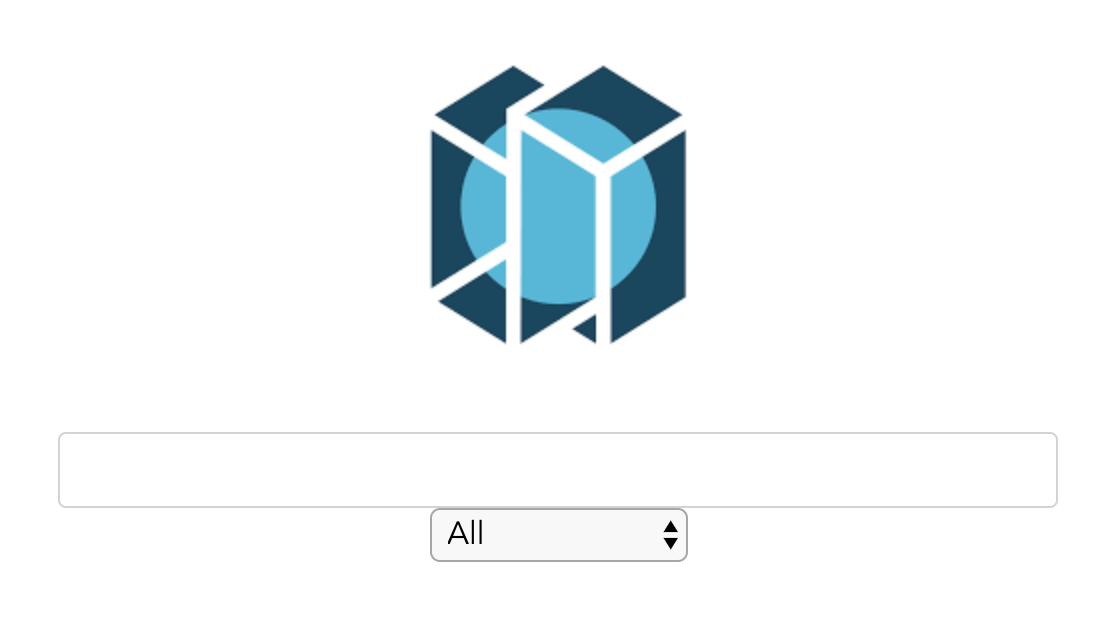
\includegraphics[width=0.5\textwidth]{figures/DashboardMain.png}
	\caption{Main screen of the dashboard}
	\label{fig:dashboard-main}
\end{figure}


The main screen of the dashboard is shown on \autoref{fig:dashboard-main}.


\section{Improvement of Recommendations via Feedback Learning}

\section{Conclusion}

% TODO: add more chapters here

\appendix{}

\microtypesetup{protrusion=false}
\listoffigures{}
\listoftables{}
\microtypesetup{protrusion=true}
\printbibliography{}

\end{document}
